% !TeX spellcheck = en_US
%MEGA MAN X.TEX
\chapter{Game overview}
\textit{Mega Man X} originated as a spin-off game derived from the classic Mega Man series, initially released for the Super Famicom/SNES consoles (later extended to PC) during the period spanning from 1993 to 1995~\cite{wiki:MMX}. Set a century after the events of the main series' timeline, the game unfolds in a world where both humans and robots capable of experiencing emotions coexist. In this world, the protagonist, X, is one of these special robots and finds himself engaged in a relentless battle against the evil Sigma who aims to eradicate humans to establish a world solely governed by robots.

\begin{figure}[htp]
	\centering
	\begin{subfigure}[c]{0.4\linewidth}
		\centering
		
\includegraphics[width=\linewidth]{figures/X1/mmx_cover.jpeg}
	\end{subfigure}
	\begin{subfigure}[c]{0.4\linewidth}
		\centering
		
\includegraphics[width=\linewidth]{figures/X1/mmxmh.png}
	\end{subfigure}
	\caption{Cover art for the American version of X1 and its remake.}
\end{figure}
In 2005, a remake of the game was created specifically for the PlayStation Portable. This version, known as \textit{Maverick Hunter X} or simply \mhx, featured upgraded 3D graphics. The primary objective of this remake was to retell the story of the first game, but with minor alterations. Notably, these changes included a reimagined portrait of X's relationships with the Mavericks and Sigma, aspects that were absent in the original game.

Furthermore, the level design received modifications as well, such as the locations of Dr.~Light's capsules or the arrangement of Sigma's stages, completely different from those found in the original version of the game. 

\section[Main plot]{Main plot (X)}
In the year 21XX, humans coexist harmoniously with a new breed of robots called reploids, robots possessing the unique capability to make independent decisions and experience emotions~\cite{Xcoll1:Manual_X1}. However, at times, a reploid's electric brain can malfunction, causing them to behave dangerously towards nearby humans and other reploids. When this occurs, the reploid is classified as a ``Maverick'' and must be halted, either for repairs or disposal. To address this issue, a specialized organization known as the Maverick Hunters was established with the sole purpose of dealing with mavericks. Leading this organization is Sigma, one of the most advanced reploids of his time.

The situation takes a dramatic turn when Sigma himself goes maverick, declaring war on humanity. He recruits other maverick hunters to his cause, either through persuasion or threats. In response to the escalating conflict, X, the main protagonist of our story, decides to join the fight alongside his close friend Zero on the battlefield—a highway currently under attack. However, X's progress is halted by Vile, an ex-hunter whom Sigma had released from prison. Only the timely intervention of Zero, who forces Vile to retreat, allows X to escape unharmed.

\begin{figure}[htp]
	\centering
	
\includegraphics[height=3cm]{figures/X1/Highway_end.jpg}
	\caption{Zero saving X from Vile.}
\end{figure}

The couple then decides to part ways: Zero embarks on a mission to locate the enemy fortress, while X takes on the task of confronting Sigma's mavericks gaining new powers and strength along the way. Eventually, he reunites with Zero, who had located Sigma's fortress flying over the sea. However, upon reaching the fortress's entrance, they are immediately faced with Vile and his formidable ride armor. Zero courageously challenges Vile in a one-versus-one battle, but is ultimately captured. Subsequently, Vile also manages to trap X, rejoicing over his apparent triumph. At this critical moment, Zero seizes an opportunity to break free from his confinement, attaching himself to the ride armor and detonating, destroying the armor but sparing Vile. Witnessing Zero's sacrifice, X finds new determination, empowering him to break free as well. He confronts Vile, now vulnerable, and successfully defeats him in battle.

Before proceeding further, X heeds Zero's final words~\cite{wiki:MMX_script}. Zero reveals to X that his auto-repair system is incapable of handling all the damages he sustained during the battle, and also that he believe X to possess a power even greater than his own, rendering him capable of facing Sigma. Eventually, Zero also entrusts his own Z-buster to X in case he had not managed to acquire the buster upgrade himself.

\begin{figure}[htp]
	\centering
	
\includegraphics[height=3cm]{figures/X1/Zero_cannon.jpg}
	\caption{Zero, near death, giving X his arm cannon.}
\end{figure}

Following Zero's demise, X continues his mission and infiltrates Sigma's fortress and confronts its dangers, including re-facing all the previously defeated mavericks. Eventually, X arrives at Sigma's lair, where the villain awaits. Sigma initially displays arrogance, being surprised that X managed to reach him and claiming he could easily destroy him. However, Sigma decides to let his pet Velguarder deal with X as he watches the fight unfold. X proves his skill by successfully defeating Velguarder, which changes Sigma's perspective a bit, understanding why Zero placed his trust in X and acknowledging that X could have been an hunter as strong as he was. Sigma then faces X himself, but ultimately X emerges victorious, destroying all Sigma's body but his head. Sigma's head then combines with a giant wolf-based mechaniloid, providing him with a new body to continue the battle against X. Despite Sigma's tenacity, however, X manages to destroy the new body too, effectively putting an end to Sigma. 

Just as the fights end, the fortress begins to explode, while Sigma blames X for shattering his dream of a world exclusively for reploids. The fortress's imminent destruction forces X to teleport to safety outside. Contemplating the consequences of the destruction he has witnessed and the sacrifices made for victory, X questions if fighting was the right choice, wondering if an alternative path could have been taken. As the flying fortress sinks into the ocean, X realizes that he will face more battles before finding the answers he seeks. After that, the game's credits roll, but an unexpected twist emerges. A message from Sigma reveals that his spirit is still intact, awaiting the construction of a new body to challenge X once again. 
\begin{figure}[htp]
	\centering
	
\includegraphics[height=3cm]{figures/X1/Ending.jpg}
	
\includegraphics[height=3cm]{figures/X1/sigma_message.jpg}
	\caption{Sigma's fortress falling in the ocean and Sigma's final message to X.}
\end{figure}

\section{Main Plot (\mhx)}
While Maverick Hunter X largely follows a similar plot to the original Mega Man X game, it does introduce some divergences, particularly concerning the relationships between characters and X's background~\cite{wiki:MM_MHX}. One of the significant points of divergence pertains to X's backstory before the commencement of the war. Below is a summary of the differences between \textit{Maverick Hunter X} and Mega Man \x:


\begin{itemize}
	
\item In-depth background: The ``Day of $\Sigma$'' OVA provides a comprehensive background of the war, explaining how Sigma initiated his revolution. In this version, X's background is altered, and he is already a Maverick Hunter before the war's beginning. He serves in the 17th Elite Unit alongside Zero, under command of Sigma himself. X holds a B hunter rank, which differs from Zero's SA rank, due to his pacifist nature and preference for dialogue over combat. Many mistake these traits for weakness, but Zero and Sigma recognize X's true potential.

\item Expanded background for Vile: Vile's character receives additional depth in Maverick Hunter X. Here, he aims to destroy both X and Sigma, seeking to create his own world. As a result, he follows Sigma's plans merely because they align with his own objectives.

\item Differences in the final portion of the story: Maverick Hunter X diverges in the final level's layout and story progression~\cite{wiki:MM_MHX_script}. Unlike the original game, where X and Zero immediately confront Vile upon entering Sigma's fortress, here X first traverses the whole fortress, encountering previously defeated bosses resurrected to challenge him. Only at the end X does meet with Zero and encounters Vile. As in the main story, Vile captures both of them, leading to Zero's sacrifice and X ultimately defeating Vile.

\item Sigma's attitude toward X: In Maverick Hunter X, Sigma already suspects X's immense potential. He tests X by making him fight Velguarder, rather than assuming Velguarder alone would be enough to defeat X, as in the original game. Sigma then confronts X directly, leading to the same outcome as in the original story.

\end{itemize}


\section{Main Characters}
\subsection{X}
\begin{figure}[htp]
	\centering
	
\includegraphics[height=\portraitsize]{figures/X1/X_X1.png}
	\caption{X}
\end{figure}

X, as described in Chapter~\ref{char:X}, is the first of a new generation of sentient robots created by Dr.~Thomas Light in the year 20XX. X possesses the unique ability to experience emotions and make autonomous decisions, but due to his immense power, Dr.~Light needed to conduct a series of tests to ensure his integrity. Unfortunately, Dr.~Light's own lifespan would not permit him to complete all the tests, so he sealed X in a capsule capable of running the tests automatically.

In the year 21XX, during an archaeological expedition, Dr.~Cain (chapter~\ref{char:Cain}) discovers X's capsule~\cite{X:Manual,wiki:Cain_journal}. Dr.~Cain reawakens X and, with the aid of Light's designs and X's assistance, begins developing a new type of robot called ``Reploids''. The reploids quickly become integrated into society and prove invaluable in performing challenging tasks. Despite this, however, X remains uncertain about his place in the world and the future that Dr.~Light envisioned for him. However, when the villainous Sigma initiates a war against humanity, X is compelled to step forward and fight alongside his ally, Zero, to restore peace.

The account given so far aligns with X's original role in the original game. However, as mentioned earlier, Maverick Hunter X rewrites X's backstory, introducing a different series of events before Sigma's revolt. In this retelling, Dr.~Light seals X away not to test his integrity but because he believes the world is not yet ready for X's technology and potential. Still, Dr.~Light firmly believes that X possesses a good spirit and that he will use his power to achieve peace~\cite{wiki:MM_MHX_X}. Furthermore, upon awakening, X joins immediately the Maverick Hunters (a deviation from the original storyline), serving in the 17th Elite Unit alongside Zero and under Sigma's direct command. Despite X's extraordinary potential, his hunter rank is designated as B, unlike Zero's SA rank. This low rank is attributed to X's apparent hesitation during battle, a result of his pacifist nature, which makes him reluctant to fight and prevents him from fully utilizing his true power~\cite{Xcoll1:Manual_X1}. Nevertheless, when Sigma launches his war against humanity, X decides to stand up and fight alongside Zero to restore peace to the world.

\subsection{Zero}
\begin{figure}[htp]
	\centering
	
\includegraphics[height=\portraitsize]{figures/X1/Zero_X1.png}
	\caption{Zero}
\end{figure}

In the original Mega Man X1 game, very little information is provided about Zero (more details in chapter~\ref{char:Zero}), other than the fact that he is a friend of X and the new leader of the Maverick Hunters~\cite{X:Manual} after Sigma's defection, holding the highest rank among all remaining hunters. Maverick Hunter X delves deeper into Zero's relationship with X, portraying him as a close friend and mentor to X in the 17th Elite Unit, serving under Sigma and holding an SA hunter rank. Zero is depicted as a resolute fighter who firmly opposes evil, showing no mercy when facing Mavericks, even if they include Sigma himself~\cite{Xcoll1:Manual_X1}.

Despite these differences in character portrayal, Zero's story remains consistent between both games. He first appears at the end of the highway, rescuing X from Vile's grasp and requesting X to handle Sigma's forces while he searches for the enemy hideout. Later, Zero is spotted at the entrance of Sigma's fortress, acting as a diversion to enable X to infiltrate the fortress undetected. Finally, Zero is present during the final showdown with Vile, where he sacrifices himself to destroy Vile's armor, enabling X to defeat him. In his final moments, Zero imparts crucial words to X, urging him to go and confront Sigma. He even gives X his own Z-buster as a backup, in case X hasn't upgraded his own buster yet.

\section{Game Mechanics}
\textit{Mega Man X}'s gameplay remains true to its original series, offering a 2D hybrid experience combining run'n'gun mechanics with platforming elements where the main protagonist, X, must complete different stages to unlock the final area of the game. Each stage has its own distinct theme and contains specific items to collect. Some of these items may require X to obtain other power-ups first, typically acquired from defeating bosses in the game. At the end of each stage a boss awaits, and defeating him grants X a new weapon based on one of its attacks. Like in the original series, X can access all the main stages in any order, and each boss has a corresponding ``weak point'' vulnerable to a weapon obtained from defeating another boss. Such weakness can be exploited to deal more damages to the boss, but in some occasion they can also stun them or disabling certain bosses' attacks.

Mega Man X1 introduces several new mechanics that will define the series~\cite{wiki:X1_features}:
\begin{itemize}
	
\item \textbf{Dash}: X can dash and move faster, as well as perform dash-jumps with the leg parts. This mechanic is an evolution of the sliding mechanism from the original series, as it is now tied to a specific button.

\item \textbf{Wall-jumping}: X gains the ability to jump onto walls to climb them, as well as slide down for controlled descent. He can also dash-jump off walls to cover greater distances.

\item \textbf{Armor parts}~[\ref{X1:Armor}]: By discovering Dr.~Light's capsules (four in total), X can be upgraded and unlock new powers that aid the player during the game.

\item \textbf{Sub-Weapon} charging~[\ref{X1:sub_weapon}]: With the buster upgrade, X can not only charge his primary X-buster, as in the main series, but he can also charge his other sub-weapons to increase damage or alter their functionality.

\item \textbf{Heart tanks}: In addition to the classical Sub-tank, eight heart tanks are scattered across various stages, one per stage. Picking them up increases X's energy capacity by two, starting from 16 and reaching a maximum of 32~\cite{stratwiki:Heart_tank}.

\item \textbf{Stage interactions}: Although limited, beating certain stages can affect others and change them in some portions
\end{itemize}

\section{Weapons}\label{X1:sub_weapon}
Here is a list of all sub-weapons available in\textit{ Mega Man X}/ \textit{Mega Man Maverick Hunter X} (\cite{MHX:manual}, \cite{wiki:X_weapons}):

\subsection{
\includegraphics[width=12px, height=10px]{figures/X1/weapons/Homig_T.jpg} Homing Torpedo}\label{Homing_torpedo}
When X equips this sub-weapon, he gains the ability to fire up to two torpedoes (three in Maverick Hunter X)~\cite{wiki:Homing_torpedo}. These torpedoes possess the unique characteristic of tracking enemies. As they accelerate, they automatically target the nearest enemy and follow its movements. When charged, X can release a fan of four fish-shaped missiles (six in Maverick Hunter X). These charged missiles exhibit increased speed and attack power, making them more effective homing projectiles against enemies. Players obtain this powerful weapon after defeating Launch Octopus~[\ref{boss:Launch_octopus}].

\begin{figure}[htp]
	\centering
		
\includegraphics[height=3cm]{figures/X1/weapons/Homing_torpedo_1.jpg}	
		
\includegraphics[height=3cm]{figures/X1/weapons/Homing_torpedo_2.jpg}	
	\caption{Homing Torpedo sub-weapon's regular and charged attack.}
\end{figure}

\subsection{
\includegraphics[width=12px, height=10px]{figures/X1/weapons/C_sting.jpg} Chameleon Sting}\label{Chameleon_sting}

The Chameleon Sting, acquired after defeating Sting Chameleon~[\ref{boss:Sting_chameleon}], functions by emitting a single laser that subsequently splits into three directions: forward, up-forward, and down-forward. However, in Maverick Hunter X, the weapon directly emits three lasers, which can be angled diagonally upward and downward and have slightly increased speed. In both versions of the game, when the weapon is charged, X flashes in various rainbow colors, granting him temporary invincibility to all damage (except for instant-kill hazards like pits) for a brief period. In the original game X is unable to switch to any other weapon while the invincibility is active. However, in the remake, he has the freedom to fire with the current weapon and use any other weapon simultaneously~\cite{wiki:Chameleon_sting}. 
\begin{figure}[htp]
	\centering
		
\includegraphics[height=3cm]{figures/X1/weapons/Chameleon_sting.jpg}
	\caption{Chameleon Sting sub-weapon}
\end{figure}

\subsection{
\includegraphics[width=12px, height=10px]{figures/X1/weapons/Rolling_S.jpg} Rolling Shield}\label{Rolling_shield}
After defeating Armored Armadillo~[\ref{boss:Armored_Armadillo}], X acquires the Rolling Shield. With this weapon, X spins energy at high speeds within the X-Buster and launches it as an energy shot that rolls along the ground. The resulting projectile is approximately the same size as X (half its size in Maverick Hunter X) and will continue rolling along the ground until it makes contact with an enemy or disappears after a while. If the shield comes into contact with a wall, it ricochets once and then disappear upon hitting a wall again. Only in Maverick Hunter X, the Rolling Shield possesses the additional abilities to absorb incoming projectiles directed toward it and to take out Mets even when they are hiding~\cite{wiki:Rolling_shield}. 

When charged, X can surround himself with an energy field that eliminates any enemy with less than three hit points upon contact. However, the energy field will disappear upon hitting enemies with more than that amount of life. In the original game, while the charged shield is active, X cannot shoot or change weapons in-game. To change weapons, the player must access the pause menu, causing the shield to disappear.

\begin{figure}[htp]
	\centering
		
\includegraphics[height=3cm]{figures/X1/weapons/Rolling_shield_1.jpg}	
		
\includegraphics[height=3cm]{figures/X1/weapons/Rolling_shield_2.jpg}	
	\caption{Rolling Shield sub-weapon's regular and charged attack.}
\end{figure}

\subsection{
\includegraphics[width=12px, height=10px]{figures/X1/weapons/F_wave.jpg} Fire Wave}\label{Fire_wave}
The Fire Wave transforms X's buster into a powerful flamethrower, capable of dealing continuous damage to enemies, but at the price of not being able of using it underwater.\begin{figure}[htp]
	\centering
	
\includegraphics[height=3cm]{figures/X1/weapons/Fire_wave_1.png}
	
\includegraphics[height=3cm]{figures/X1/weapons/Fire_wave_3.png}
	
\includegraphics[height=3cm]{figures/X1/weapons/Fire_wave_2.png}
	
\includegraphics[height=3cm]{figures/X1/weapons/Fire_wave_4.jpg}
	\caption{Fire Wave sub-weapon's regular and charged attack both outside and inside water.}
\end{figure} Upon pressing the fire button, X releases a continuous stream of fire from his X-buster, draining energy in the process. When the weapon is fully charged, X launches a fireball that creates a pillar of fire upon hitting the ground, and it moves forward for a certain distance.
 To charge the weapon, X must continue firing, causing energy to deplete in the process. If used underwater, the weapon becomes ineffective, producing only smoke (but still consuming energy). Players obtain the Fire Wave after defeating Flame Mammoth~[\ref{boss:Flame_mammoth}].



\subsection{
\includegraphics[width=12px, height=10px]{figures/X1/weapons/Storm_T.jpg} Storm Tornado}\label{Storm_tornado}

The Storm Tornado transforms the X-buster into a powerful fan that unleashes hard-hitting winds, capable of destroying enemies in its path. When fired, it shoots a horizontal tornado that remains on the screen for a brief period before starting to move in the direction X was facing when it was shot. Due to its length, the tornado can hit enemies multiple times, making it an effective way to dispose of most foes, especially larger ones. In Maverick Hunter X, the length of the Storm Tornado is halved, allowing it to shoot at a faster rate.

When the Storm Tornado is charged, it creates a large vortex that covers the entire screen in height. In the original game, this vortex surrounds X himself, while in the remake, it instead explodes from the shot projectile once it hits a solid surface~\cite{wiki:Storm_tornado}. Players obtain the Storm Tornado by defeating Storm Eagle~[\ref{boss:Storm_Eagle}]. 
\begin{figure}[htp]
	\centering
		
\includegraphics[height=3cm]{figures/X1/weapons/Storm_tornado_1.jpg}
		
\includegraphics[height=3cm]{figures/X1/weapons/Storm_tornado_2.jpg}
	\caption{Storm Tornado sub-weapon's regular and charged attack.}
\end{figure}

\subsection{
\includegraphics[width=12px, height=10px]{figures/X1/weapons/E_Spark.jpg} Electric Spark}\label{Electric_spark}
The Electric Spark creates high-pressure voltage within the X-Buster and fires it, allowing for a maximum of three shots at a time. When the electric spark hits a hard surface, it splits in half and starts traveling up and down along the surface.

In the original Mega Man X, when this weapon is charged, X releases two electric columns in front and behind him, which moves in their respective directions. On the other hand, in Maverick Hunter X, the weapon generates electricity in all directions starting from X's body, covering the entire screen. 

Players obtain the Electric Spark upon defeating Spark Mandrill~[\ref{boss:Spark_mandrill}].

\begin{figure}[htp]
	\centering
		
\includegraphics[height=2cm]{figures/X1/weapons/Electric_spark_1.jpg}
		
\includegraphics[height=2cm]{figures/X1/weapons/Electric_spark_2.jpg}
		
\includegraphics[height=2cm]{figures/X1/weapons/Electric_spark_3.jpg}
	\caption{Electric Spark sub-weapon's regular (normal and split) and charged attack.}
\end{figure}

\subsection{
\includegraphics[width=12px, height=10px]{figures/X1/weapons/B_cutter.jpg} Boomerang Cutter}\label{Boomerang_cutter}

Upon defeating Boomer Kuwanger~[\ref{boss:Boomer_Kuwanger}], X gains access to the Boomerang Cutter. This unique weapon fires up to three sharp boomerangs~\cite{wiki:Boomerang_cutter} made from a special metal. The trajectory of these boomerangs depends on X's position when he fires them: they arc upwards if X is standing on the ground and arc downwards if X is in the air. If a boomerang fails to hit an enemy, it returns to X, and if it passes a collectible on its way back, it picks up the item and delivers it to X, even retrieving dropped life or weapon energy from defeated enemies. If a boomerang successfully returns to X without hitting an enemy, it replenishes the energy used to create it. When charged, X releases four larger boomerangs that spiral out of him diagonally. In Maverick Hunter X, this has been altered to four boomerangs of doubled size that move back and forth in a straight line a few times.

Additionally, the Boomerang Cutter has a special perk when used against Flame Mammoth and Launch Octopus. While such enemies are not heavily damaged by the weapon, hitting Flame Mammoth will cause hit to lose his trunk, whereas Launch Octopus will lose his tentacles, resulting in both bosses being unable to perform certain attacks anymore.

\begin{figure}[htp]
	\centering
		
\includegraphics[height=3cm]{figures/X1/weapons/Boomerang_1.jpg}
		
\includegraphics[height=3cm]{figures/X1/weapons/Boomerang_2.jpg}
	\caption{Boomerang Cutter sub-weapon's regular and charged attack.}
\end{figure}

\subsection{
\includegraphics[width=12px, height=10px]{figures/X1/weapons/S_ice.jpg} Shotgun Ice}\label{Shotgun_ice}

Shotgun Ice is the weapon that X acquires after defeating Chill Penguin~[\ref{boss:Chill_Penguin}]. This powerful weapon absorbs moisture from the air and fires it in crystallized form which, upon hitting an enemy or a hard surface, shatter into five pieces that ricochet backward. If these ice fragments collide with another wall or enemy, they are destroyed. When charged, the weapon has a different effect in the original game and its remake. In Mega Man X1 the charged Shotgun Ice creates a Chill Penguin-shaped ice platform, resembling the ice sculpture that the boss can create. X can stand on this platform, and it starts moving forward shortly after being created. However, in Maverick Hunter X, the charged version only creates a sharp sled of ice without any decorative shape.

A notable quirk in Mega Man X1 is that if X creates the platform and then positions himself in the same spot where the platform is forming (due to the platform's delayed creation), the platform will slightly push X left or right based on its position. This can lead to glitches such as wall clipping, allowing X to pass through walls in certain circumstances (section \ref{X1:misc}). This glitch is not present in Maverick Hunter X.

\begin{figure}[htp]
	\centering
		
\includegraphics[height=2.4cm]{figures/X1/weapons/Shotgun_ice_1.jpg}
		
\includegraphics[height=2.4cm]{figures/X1/weapons/Shotgun_ice_2.jpg}
		
\includegraphics[height=2.4cm]{figures/X1/weapons/Shotgun_ice_3.jpg}
	\caption{Shotgun Ice sub-weapon's regular (normal and deflected shots) and charged attack.}
\end{figure}

\section{First Armor}\label{X1:Armor}

While exploring stages, X may come across one of the four capsules hidden by Dr.~Light. When X comes into contact with a capsule, it opens, revealing Dr.~Light's hologram, which will speak to X and present him with one of the armor parts~\cite{wiki:First_armor}, providing an explanation of how the specific armor part functions. 
\begin{figure}[htp]
	\centering
	
\includegraphics[height=\portraitsize]{figures/X1/First_armor.png}
	\caption{First armor X.}
\end{figure}

The First Armor is comprised of four parts (plus a secret extra one), each offering unique enhancements to X's abilities:
\begin{itemize}
\item \emph{Foot Parts}: The ``\textit{Emergency Acceleration System}''~\cite{X:Manual} allows X to dash forward, perform dash-jumps, and execute wall dash-jumps. While dashing, X's hitbox's height is reduced slightly. Additionally, X can destroy specific blocks by wall-jumping onto them. In the original Mega Man X, the capsule containing the foot parts is located in the middle of the Snow Mountain Stage and is mandatory to obtain. However, in Maverick Hunter X, the capsule is moved to the beginning of the Factory Stage.

\item \emph{Body Parts}: Equipping the Body Parts reduces all incoming damage to X by 50\%. In the original game, the capsule is found in the Forest stage after climbing the wall right before the cave. After defeating RT-55J, the capsule will emerge from the ground. In Maverick Hunter X, the Body Parts are moved to the Storm Eagle Stage, requiring the Head Parts to access them.

\item \emph{Arm Parts}: The Arm Parts allow X's X-Buster to be charged up to a third level and enable charging of special weapons. Dr.~Light originally intended this upgrade to be included in the basic X-Buster~\cite{X:Manual}, but he sealed away X before it was ready, making it a separate modification given to X later. While the capsule itself is not mandatory, if the player faces Vile without finding the capsule first, the game will still grant them the buster upgrade in the form of the Z-Buster. In Maverick Hunter X, the Arm Parts unlock the Spiral Crush Buster, which is a larger version of the second-level charged shot and hits multiple times, while the Z-Buster deals more damage against bosses than the previous alternative. In Mega Man X, the capsule is located in the Factory stage, requiring a precise dash-jump and the Head Parts to break some blocks in the ceiling. In the remake, it is in the same place where the Body Parts were in the original game.
\begin{figure}[htp]
	\centering
	
\includegraphics[height=2cm]{figures/X1/weapons/Buster_4.jpg}
	\caption{Spiral Crusher Buster}
\end{figure}
\item \emph{Head Parts}: Equipping the Head Parts grants X the ability to break specific blocks with a headbutt and avoid damage from falling rocks in the Forest stage. In the original game, the capsule is found in the Airport stage, hidden behind an obstacle marked with a flammable warning, which can be destroyed simply by shooting at it. In the remake, it is in Chill Penguin's stage, requiring the foot part to break blocks hiding it.

\item \emph{Hadoken}: While not technically a part of the First Armor, it is a hidden upgrade stored inside a Light's capsule. This technique allows X to perform the well-known move from Street Fighter by inputting the button combination $\downarrow$ $\searrow$ $\rightarrow$ + fire button  (with X facing right)  or using the same combination while X is charging and releases the charged shot~\cite{RTA_wiki:X1}, provided that X is at full health. The projectile deals 32 points of damage~\cite{wiki:Hadoken} to all enemies, essentially one-shotting every non-shielded enemy, including bosses. The only exception is Sigma's final form, but this limitation exists only in the original Mega Man X. In both the original game and its remake, the capsule containing the Hadoken is hidden in Armored Armadillo's stage. It's worth noting that in the original game, the Hadoken power-up is not saved by the password system, meaning it has to be unlocked again if the game is restarted. However, in the remake, Maverick Hunter X, this limitation is not present.
\begin{figure}[htp]
	\centering
	
\includegraphics[height=2cm]{figures/X1/weapons/Hadoken.jpg}
	\caption{Hadoken}
\end{figure}

\end{itemize}

\chapter{Stages}

\section{Highway (Introduction Stage)}

The Highway Stage, also known as Central Highway in \textit{Maverick Hunter X}, serves as the first stage of the game. X arrives here to join the fight against Sigma's forces. The stage serves as a straightforward introduction, where X travels through it while eliminating different enemies and learning basic mechanics such as wall-jumping. The stage can be divided into two main sections~\cite{stratwiki:HighWay}, with the second one featuring more hazards such as gaps and falling pieces of the highway (indicated by a darker texture color).

In the first section of the highway, two sub-bosses in the form of \hyperlink{miniboss:Bee_Blader}{Bee Bladers} are encountered. At the end of the stage, X faces the \hyperlink{vehicle:Death_Rogumer}{Death Rogumer}, which sends several \hyperlink{enem:Road_Attackers}{Road Attackers} towards him. After some of these enemies have been destroyed Vile appears, dropping from  airship, and starts attacking X with his ride armor.\begin{figure}[htp]
	\centering
	
\includegraphics[height=3cm]{figures/X1/Highway_screenshot.jpg}
	\caption{X facing Vile.}
\end{figure} It's important to note that Vile is invincible during this encounter, so fighting back is futile. As X's health drops below a certain threshold, Vile will begin shooting an energy projectile towards X. If the projectile hits X, he will become trapped and the fight will end, leading to the cutscene where Zero comes to rescue X. In speedruns, players tend  to start this fight with low health, which forces Vile to immediately shoot the trapping projectile, effectively skipping the entire fight. Caution is, however, required, as Vile will continue attacking with his ride armor, potentially defeating the player if not careful.

This stage contains following enemies~\cite{wiki:Highway}:
\begin{itemize}
	\item \hyperlink{enem:Ball_De_Voux}{Ball De Voux}
	\item \hyperlink{enem:Bomb_Been}{Bomb Been}
	\item \hyperlink{enem:Crusher}{Crusher}
	\item \hyperlink{enem:Gun_Volt}{Gun Volt}
	\item \hyperlink{enem:Jamminger}{Jamminger}
	\item \hyperlink{enem:Road_Attackers}{Road Attackers}
	\item \hyperlink{enem:Spiky}{Spiky }
	\item \hyperlink{miniboss:Bee_Blader}{Bee Blader }
\end{itemize}
\begin{figure}[htp]
	\centering
	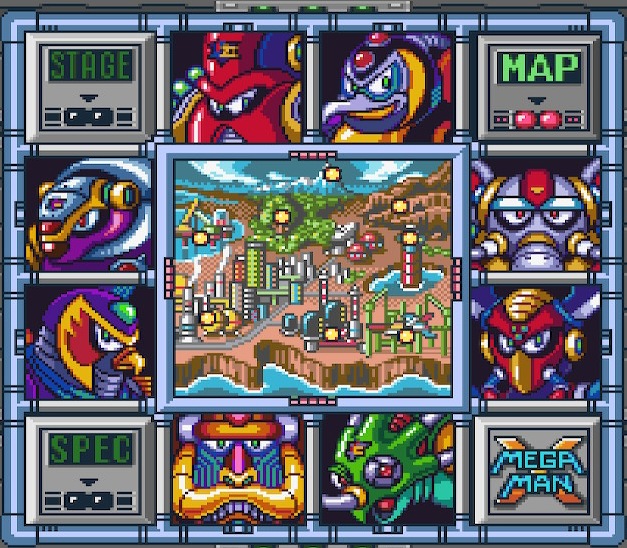
\includegraphics[height=4cm]{figures/X1/Full_map.png}
	\caption{Full map with Bosses and their locations}
\end{figure}
After completing the introduction stage, the player is presented with the classic boss selection screen typical of the Mega Man franchise. 


\section{Ocean}

The Ocean Stage, later renamed Subterranean Base in \textit{Maverick Hunter X}, is where Launch Octopus hides. The stage begins at the shoreline before X immerses underwater shortly after. Underwater, X gains the ability to jump higher, and skilled players can use this in combination with dash-jumping to skip a significant portion of the stage's first part~\cite{stratwiki:Ocean}. Various fish-based enemies populate the stage, but the main challenges come from the sub-bosses, three in total plus an optional one.

In the first part of the stage, players face difficulties from spiked pits that X must jump over. \hyperlink{enem:Sea_Attacker}{Sea Attackers} will spawn in groups of three from these pits, interrupting X's jumps and potentially causing him to fall into the spikes. Additionally, there are two \hyperlink{miniboss:Anglerge}{Anglerge} sub-bosses that make this section challenging. The second Anglerge is particularly dangerous because it will try to push or pull X into the spiked pits on the floor using its vacuum attack. Players can adopt a strategy of staying on the leftmost platform, dashing to the right when the Anglerge starts pulling, then shooting while it pushes X. Anglerges will also shoot serpent-shaped harpoons horizontally, which will then move vertically to hit X when above or below him. Occasionally, they will also shoot a beam of light from their lamp, which can be destroyed.

After passing the second sub-boss, the second part of the stage begins. Here, spiked gaps are less common, but whirlpools appear at regular intervals and specific positions, propelling X up to the ocean's surface if he gets caught in them. As X proceeds, bombs dropped by a \hyperlink{miniboss:Cruiziler}{Cruiziler} enemy will start falling from above. Players can either climb a whirlpool to get onto the Cruiziler and destroy its core, stopping it from shooting bombs, or they can avoid it and continue through the level. Moving forward, X will encounter an arena filled with sand, where an \hyperlink{miniboss:Utuboros}{Utuboros} will attack by rising from the sand, swimming for a while, and then submerging again. This enemy is invincible for most of its body, with only the head and tail being vulnerable. Although its weakness is considered to be the Boomerang Cutter, players can use the Storm Tornado to destroy it in one shot by firing it from behind its head ~\cite{wiki:Utuboros}. After defeating this sub-boss, and moving forward, X will reach the boss door.

Here is a list of all enemies present in the stage~\cite{wiki:Ocean}:
\begin{itemize}
	\item \hyperlink{enem:Amenhopper}{Amenhopper}
	\item \hyperlink{miniboss:Anglerge}{Anglerge}
	\item \hyperlink{miniboss:Cruiziler}{Cruiziler}
	\item \hyperlink{enem:Gulpfer}{Gulpfer }
	\item \hyperlink{enem:Mega_Tortoise}{Mega Tortoise }
	\item \hyperlink{enem:Sea_Attacker}{Sea Attacker}
	\item \hyperlink{enem:Sky_Claw}{Sky Claw }
	\item \hyperlink{miniboss:Utuboros}{Utuboros}
\end{itemize}

\subsection{Heart Tank}
This stage only hides a heart tank. In order to get it the player must first destroy the Cruizer by reaching the ocean's surface via a whirlpool to destroy its core, avoiding in the process the Sky Claws spawned by the ship. Once destroyed, the Cruizer will sink and  destroy the ocean's floor, revealing an hidden portion with a large room filled with spikes on the ground. Here an Utuboros  must be defeated to open the door which leads to a Heart Tank. 
\begin{figure}[htp]
	\centering
	\begin{subfigure}{0.32\textwidth}
		\centering
		
\includegraphics[height=2.5cm]{figures/X1/Launch_octopus/Octopus_heart_1.jpg}
		\caption{}
	\end{subfigure}
	\begin{subfigure}{0.32\textwidth}
		\centering
		
\includegraphics[height=2.5cm]{figures/X1/Launch_octopus/Octopus_heart_2.jpg}
		\caption{}
	\end{subfigure}
	\begin{subfigure}{0.32\textwidth}
		\centering
		
\includegraphics[height=2.5cm]{figures/X1/Launch_octopus/Octopus_heart_3.jpg}
		\caption{}
	\end{subfigure}
	\caption{(a)Via whirlpool the player can reach the Cruizer on ocean's surface,(b) When destroyed the ship will fall and break the ocean floor (c) Once destroyed the Utuboros inside the cave, a room will open with the Heart Tank inside}
\end{figure}

\subsection{Launch Octopus}\label{boss:Launch_octopus}

Launch Octopus, also known as the ``\textit{General of the Deep Sea}''~\cite{book:MMX_Complete_art} was originally a Maverick Hunter of the 6th Fleet armada before joining Sigma's rebellion and setting his base in the dept of the Ocean, in order to attack marine cities and cut off shipping routes. In the original Mega Man X game, he sided with Sigma because he shared the dream of a world only for reploids and was dubious about protecting humans. However, in Maverick Hunter X, he is portrayed as a military tactician who seeks beauty in combat and considers himself an unappreciated artist of underwater fighting. Only Sigma understood his art, leading Launch Octopus to join him~\cite{wiki:MM_MHX_script}.
\begin{figure}[htp]
	\centering
	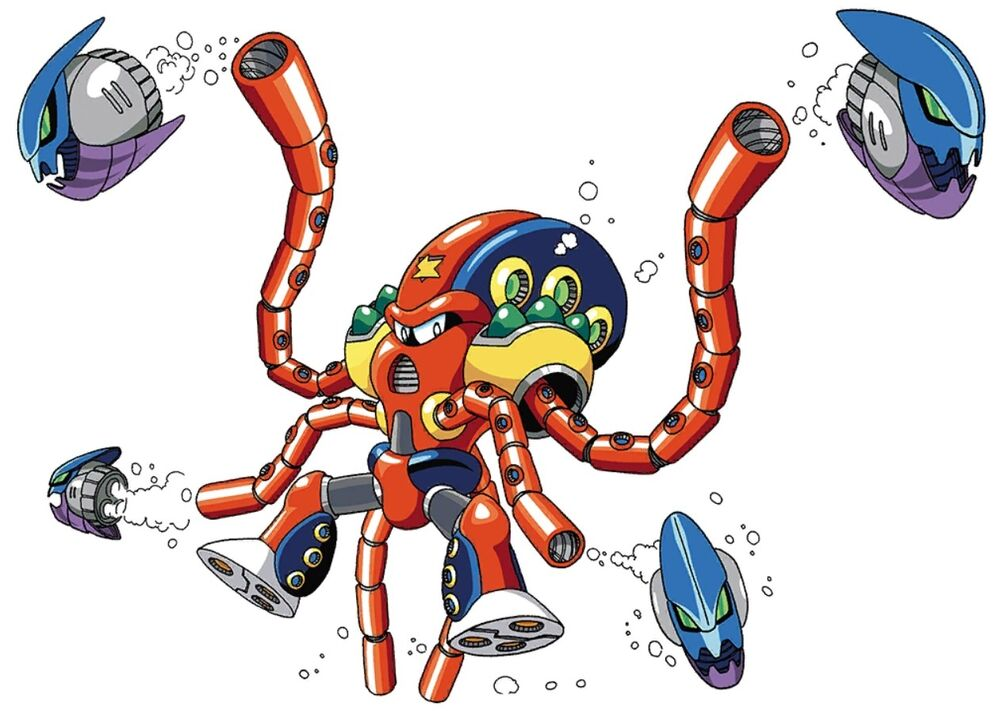
\includegraphics[height=\portraitsize]{figures/X1/Launch_octopus/LaunchOctopus.jpg}
	
\includegraphics[height=\portraitsize]{figures/X1/Launch_octopus/MHXLaunchOctopus.jpg}
	\caption{Launch Octopus' designs (\cite{book:MMX_Complete_art})}
\end{figure}

During the boss battle, Launch Octopus has three main techniques: the \emph{Homing Torpedo}, a charged version of the previous attack (which is faster and more powerful), and the \emph{Energy Drain}.  Octopus often starts the fight with a barrage of homing missiles, to then switch to one of his other two attacks. Notably all version of his homing missiles can be destroyed by shooting at them. His Energy Drain attack involves him swimming in the upper left or right corner, spinning to create a whirlpool to suck X in and drain his energy to replenish his own.
\begin{figure}[htp]
	\centering
	\begin{subfigure}{0.48\textwidth}
		\centering
		
\includegraphics[height=2.5cm]{figures/X1/Launch_octopus/Octopus_missile.jpg}
		\caption{Homing Torpedo}
	\end{subfigure}
	\begin{subfigure}{0.48\textwidth}
		\centering
		
\includegraphics[height=2.5cm]{figures/X1/Launch_octopus/Octopus_piranha.jpg}
		\caption{Charged Homing Torpedo}
	\end{subfigure}

	\begin{subfigure}[c]{0.15\textwidth}
		\centering
		
\includegraphics[height=3cm]{figures/X1/Launch_octopus/Octopus_vortex.jpg}
		\caption{Vortex}
	\end{subfigure}
	\begin{subfigure}[c]{0.22\textwidth}
		\centering
		
\includegraphics[height=3cm]{figures/X1/Launch_octopus/Octopus_drain.jpg}
		\caption{Energy Drain}
	\end{subfigure}
	\begin{subfigure}[c]{0.4\textwidth}
		\centering
		
\includegraphics[height=3cm]{figures/X1/Launch_octopus/Octopus_cut.jpg}
		\caption{Tentacles cut off}
	\end{subfigure}
	\caption{Launch Octopus' attacks~\cite{wiki:Launch_octopus,book:Compendium}}
\end{figure}
Octopus main weakness is the Rolling Shield, which deals extra damage to him. The Boomerang Cutter is also effective weapon, as it can sever his tentacles in three hits, preventing him from using his Energy Drain attack. Upon defeating Launch Octopus, X gains the Homing Torpedo weapon (\ref{Homing_torpedo}). Additionally, this victory causes a flood in the Forest Stage, resulting in water appearing near the beginning of that stage.

In terms of his official measurements, Launch Octopus is listed as 232 cm tall and 182 kg heavy\cite{wayback:X_resources}, though there are discrepancies between in-game information and the official data~\cite{wiki:Launch_octopus}


\begin{figure}[htp]
	\begin{minipage}[c]{0.45\linewidth}
		\vspace{0pt}
		\centering
		\includegraphics[height=4cm]{figures/X1/Launch_octopus/Launch_octopus_specs.png}
	\end{minipage}
	\begin{minipage}[c]{0.45\linewidth}
		\centering
		\vspace{0pt}
		\begin{tabular}[h]{l c}
			\toprule
			Health Bar & 32\\
			\midrule
			\multicolumn{1}{c}{Attack} & \multicolumn{1}{c}{Damage}\\
			Contact & 4\\
			Homing Torpedo & 2\\
			Charged H. Torpedo & 2\\
			Energy Drain & 1-15\\
			\bottomrule
		\end{tabular}
	\end{minipage}
	\caption{Left: Launch Octopus' specifications and according to X1; Right: In-game data~\cite{wiki:Launch_octopus}. }
	\label{Octopus_specs}
\end{figure}


\section{Snow Mountain}

Snow Mountain, also known as the \textit{Abandoned Missile Base} in Maverick Hunter X, is often the first stage that many players choose when starting the game due to its relatively low level of danger~\cite{stratwiki:Snow_mountain} and the valuable upgrade it contains—the Foot Parts. The stage is set in a snow-covered mountain that X must climb to reach the boss.

The stage can be divided into three main areas. In the first area, X starts outside and follows a path that leads him into a cave while encountering various enemies along the way. Inside the cave (the second area), X must climb while avoiding enemies dropping from higher levels. He also needs to navigate across frozen platforms separated by pits until he reaches the end of the cave. In the third area, X returns to the outside and has the option to use a Ride Armor. With the Ride Armor, he can proceed for a while, but he will also face another enemy Ride Armor. The player can choose to keep the Ride Armor and enter a small cave, where they must jump some gaps using the armor while dealing with enemies, or they can use the Ride Armor to reach the top of the cave by jumping out of it to gain extra lift, effectively skipping the lower portion.

Afterwards, there is a tall wall that the Ride Armor cannot surpass, and X must leave it behind. Here, he follows a path full of slopes, gaps, and \hyperlink{enem:Snow_Shooter}{Snow Shooters}, which throw snowballs that become larger the longer they roll on the snowy ground. After passing these obstacles, the player will reach the boss door, where they will face the stage's boss.

The stage contains following enemies~\cite{wiki:Snow_mountain}:
\begin{itemize}
	\item \hyperlink{enem:Armor_Soldier}{Armor Soldier} (with Ride Armor)
	\item \hyperlink{enem:Axe_Max}{Axe Max}
	\item \hyperlink{enem:Batton_Bone}{Bat Bone}
	\item \hyperlink{enem:Bomb_Been}{Bomb Been}
	\item \hyperlink{enem:Flammingle}{Flammingle}
	\item \hyperlink{enem:Jamminger}{Jamminger }
	\item \hyperlink{enem:Ray_Bit}{Ray Bit}
	\item \hyperlink{enem:Snow_Shooter}{Snow Shooter}
	\item \hyperlink{enem:Spiky}{Spiky}
	\item \hyperlink{enem:Tombot}{Tombot}
\end{itemize}

\subsection{Light's Capsule}\label{X:Foot_Parts}

In the original Mega Man X, the Snow Mountain stage contains the Armor capsule for the Foot Parts. This upgrade allows X to dash, perform dash-jumps, and execute wall dash-jumps. Dashing also reduces X's height and hitbox slightly, enabling him to dodge certain attacks by dashing beneath them. The capsule is conveniently located directly on the main path after climbing the first part of the cave. Since it is placed right in the middle of the path, it cannot be avoided, making it the only mandatory capsule in the entire series.
\begin{figure}[htp]
	\centering
	\includegraphics[height=3cm]{figures/X1/Chill_penguin/Armor_foot.jpg}
	\caption{Foot Part capsule location}
\end{figure}

However, in the remake, the Snow Mountain stage hides the Head Parts instead. The capsule for the Head Parts is concealed in the first indoor climbing section and can only be accessed by breaking a block that requires the use of the Foot Parts.


\subsection{Heart Tank}\label{Penguin:heart_tank}

The stage's, Heart Tank is hidden in the last igloo X encounters before facing the section with snowballs, and to reach it X must use the Ride Armor. Passed the first igloo, there is a light blue column located just before the cave with the enemy Ride Armor,  from the top of which the player must jump with the Ride Armor and, at the maximum height, jump out of it to reach the wall leading to the upper path. On this upper path two other igloos can be found, which can be destroyed using the Fire Wave weapon. Among these igloos, the last one contains the Heart Tank that the player is seeking to collect.

\begin{figure}[htp]
	\centering
		\centering
		\includegraphics[height=3cm]{figures/X1/Chill_penguin/Chill_heart_1.jpg}
		\includegraphics[height=3cm]{figures/X1/Chill_penguin/Chill_heart_2.jpg}
	\caption{Heart Tank location.}
\end{figure}

\subsection{Chill Penguin}\label{boss:Chill_Penguin}

Chill Penguin, also known as the ``\textit{Glacial Emperor}''~\cite{book:MMX_Complete_art} was originally part of the 13th Polar Division, specifically designed to operate in polar environments due to his small size. 
\begin{figure}[htp]
	\centering
	\includegraphics[height=4cm]{figures/X1/Chill_penguin/Chill_Penguin.jpg}
	\includegraphics[height=4cm]{figures/X1/Chill_penguin/MHXChillPenguin.jpg}
	\includegraphics[height=4cm]{figures/X1/Chill_penguin/Chill_Penguin.png}
	\caption{Chill Penguin's designs~\cite{book:MMX_Complete_art} and X Dive's artwork}
\end{figure}However, due to the long permanence away from civilization, he grew tired of his mission in the South Pole and sought a way to escape. When Sigma's rebellion began, it provided Chill Penguin with the opportunity he needed to leave the South Pole and join Sigma's cause. In Mega Man X1, Chill Penguin fled  after killing his own commander, and took over a mountain base to cause chaos with avalanches~\cite{Xcoll1:Manual_X1}, while in \textit{Maverick Hunter X}, it was Sigma who brought Chill Penguin out of the South Pole and enlisted him in the 17th division~\cite{MHX:manual}, alongside a conspicuous payment to ensure his loyalty~\cite{wiki:MMX_script}, before declaring war. Penguin was known to be a belligerent and rowdy individual, sometimes showing jealousy towards Flame Mammoth due to the difference in size (\ref{boss:Flame_mammoth}).

\begin{figure}[htp]
	\centering
	\begin{subfigure}{0.4\textwidth}
		\centering
		\includegraphics[height=2cm]{figures/X1/Chill_penguin/Chill_shot.jpg}
		\caption{Shotgun Ice}
	\end{subfigure}
	\begin{subfigure}{0.42\textwidth}
		\centering
		\includegraphics[height=2cm]{figures/X1/Chill_penguin/Chill_frozen.jpg}
		\caption{X frozen near two ice statues}
	\end{subfigure}
%	\begin{subfigure}[c]{0.5\textwidth}
%		\centering
%		\includegraphics[height=2cm]{figures/X1/Chill_penguin/Chill_shatter.jpg}
%		\caption{Shotgun ice stopped by the statues}
%	\end{subfigure}
	\begin{subfigure}{0.32\textwidth}
		\centering
		\includegraphics[height=2.5cm]{figures/X1/Chill_penguin/Chill_slide.jpg}
		\caption{Slide attack}
	\end{subfigure}
%\end{figure}
%\begin{figure}
%	\centering
%	\ContinuedFloat
	\begin{subfigure}{0.3\textwidth}
		\centering
		\includegraphics[height=2.5cm]{figures/X1/Chill_penguin/Chill_blizzard.jpg}
		\caption{Blizzard attack}
	\end{subfigure}
	\begin{subfigure}{0.22\textwidth}
		\centering
		\includegraphics[height=2.5cm]{figures/X1/Chill_penguin/Chill_burn.jpg}
		\caption{Hit by fire}
	\end{subfigure}
	\caption{Chill Penguin's attacks}
\end{figure}

Chill Penguin is often considered the easiest boss of the game and the first one a player should face due the simplicity of avoiding his attacks, also thanks to the Foot Parts the stage gives to the player. He has four main attacks which he performs at random~\cite{wiki:Chill_Penguin}. When using his \emph{Shotgun Ice}, Chill Penguin will shoot four frozen projectiles which travel in a straight line, although some of them  can fall off and slide on the ground, that shatter upon contact with a wall and can nullify X's shots when the two meet. Other times instead of his projectiles he will emit his \emph{ice breath}, which will create two penguin-shaped \emph{ice statue} and freeze X if he is in the breath's range. The sculptures act both as obstacles that damage X and as covers since they blocks all projectiles, and require few shots to destroy them. 

On some occasion Chill Penguin will leap in the air and grab the hook on the ceiling, unleashing a \emph{blizzard} which will push X and the statues (if present) against a wall, causing the sculptures to shatter in the process. Finally, Penguin can also \emph{slide} on the floor, and bounce back if he hits a wall. While in this state he is invincible, but he also gets rid of the remaining sculptures.  

Since Chill Penguins attacks only cover the low part of the arena,  the best strategy use against him consists in staying on the higher ground part via continuous wall-jumps, dropping down only to hit him when vulnerable. The catch here is that sometimes Chill Penguin will perform a high jump toward X, hitting him even if he's in the high corner of the room. 

\begin{figure}[htp]
	\begin{minipage}[c]{0.45\linewidth}
		\vspace{0pt}
		\centering
		\includegraphics[height=4cm]{figures/X1/Chill_penguin/Chill_penguin_specs.jpg}
	\end{minipage}
	\begin{minipage}[c]{0.45\linewidth}
		\centering
		\vspace{0pt}
		\begin{tabular}[h]{l c}
			\toprule
			Health Bar & 32\\
			\midrule
			\multicolumn{1}{c}{Attack} & \multicolumn{1}{c}{Damage}\\
			Contact & 6\\
			Shotgun Ice & 2\\
			Ice Breath & 0\\
			Ice Statue & 4\\
			Sliding & 6\\
			\bottomrule
		\end{tabular}
	\end{minipage}
	\caption{Left: Chill Penguin's specifications and according to X1; Right: In-game data~\cite{wiki:Chill_Penguin,book:Compendium}. }
	\label{Penguin_specs}
\end{figure}

Chill Penguin's weakness is the Fire Wave, which burns and stuns him temporarily. After defeating him, X gains the Shotgun Ice weapon (\ref{Shotgun_ice}) while causing also  the lava in the Factory Stage to get frozen, making the stage less dangerous.

Chill Penguin stands at 163 cm tall and weighs 108 Kg, despite some discrepancies in the in-game information screen(\ref{Penguin_specs}).


\section{Gallery}
The Gallery Stage, also known as the \textit{Energy Mines Ruins}, is controlled by Armored Armadillo. The stage features mine carts on which X can stand and that, as soon as he boards them, they start moving along the track, increasing in speed and destroying enemies that come into contact with them. However, the player must be careful as all the carts eventually fall into pits, so X needs to jump off at the right moment to avoid falling with them. This stage is known for containing the secret Light's capsule, where X learns the Hadoken technique. It is also a good place to farm health capsules and lives.

The level itself is relatively straightforward. At the beginning, X can ride a mine cart that carries him forward and takes care of enemies until it reaches a series of gaps. After this sequence, a few small gaps and enemies stand between X and the next section, which starts with a long pit where a \hyperlink{miniboss:Mole_Borer}{Mole Borer} emerges from the left wall and chases X. The Mole Borer is invincible, and touching its roller can instantly defeat X. Players can either escape to the right to continue in the level or quickly wall jump to the left before the Mole Borer breaks the wall, and then follow it from behind (while gaining access to the sub-tank). The second part of the stage mirrors the first, with another mine cart ride at the beginning and another Mole Borer at the end. This time, however, X will land behind the Mole Borer and has to follow it as it creates a passage in the mine. The final cart ride takes the player through remaining enemies until it reaches an opening in the mountain, where it flies over a huge gap that X cannot jump across. To proceed, the player must jump off the cart to land on the other side of the pit (or grab the wall if high enough) and reach the boss door.

Following enemies are present in the stage~\cite{wiki:Gallery}:
\begin{itemize}
	\item \hyperlink{enem:Batton_Bone}{Bat Bone} 
	\item \hyperlink{enem:Batton_M-501}{Batton M-501} 
	\item \hyperlink{enem:Dig_Labour}{Dig Labour} 
	\item \hyperlink{enem:Flammingle}{Flammingle} 
	\item \hyperlink{enem:Metal_Wing}{Metal Wing} 
	\item \hyperlink{enem:Metall_C-15}{Metall C-15} 
	\item \hyperlink{miniboss:Mole_Borer}{Mole Borer}
	\item \hyperlink{enem:Spiky}{Spiky}
\end{itemize}

\subsection{Sub Tank}
\begin{figure}[htp]
	\centering
	\includegraphics[height=3cm]{figures/X1/Armored_armadillo/Armadillo_tank.jpg}
	\caption{Gallery stage's subtank location}
\end{figure}
This stage's Sub Tank is located where the first Mole Borer appears. In order to get it the player must jump into the first gap and then immediately wall-jump to the left, in order to let the Mole Borer break the wall pass beneath X. Once it has passed, the player can safely jump off and go left to find the sub tank where the Mole Borer originally was. 

\subsection{Heart Tank}
The heart tank of this stage is located near where the second Mole Borer is found. Once  X jumps off the gap he has to chase the mechaniloid and destroy it quickly, since as it proceeds it will destroy the walls needed to access to the Heart Tank. To do this the Fire Wave weapon is best option, as it deals massive amounts of damage to it in a short amount of time. 
\begin{figure}[htp]
	\centering
	\begin{subfigure}{0.2\linewidth}
		\centering
		\includegraphics[height=3cm]{figures/X1/Armored_armadillo/Armadillo_heart.jpg}
		\caption{}
	\end{subfigure}
	\begin{subfigure}{0.2\textwidth}
		\centering
		\includegraphics[height=3cm]{figures/X1/Armored_armadillo/Armadillo_heart_2.jpg}
		\caption{}
	\end{subfigure}
	\caption{Gallery stage's heart tank location. In (a) the Mole Borer has been destroyed and X can wall jump and reach it, while in (b) the Mole Borer has passed and X cannot reach the opening anymore}
\end{figure}

\subsection{Hadoken}\label{hadoken}
\begin{figure}[htp]
	\centering
	\includegraphics[height=3cm]{figures/X1/Armored_armadillo/Armadillo_hadoken.jpg}
	\caption{Hadoken capsule with Dr.Light in Ryu's attire.}
\end{figure}
The hadoken is the last upgrade X can get before facing the finals stages. The capsule containing it can be unlocked only if the player has managed to collect every other upgrade in the game: eight Heart Tanks, four Sub-Tank, four armor capsules and all the weapons from bosses. 

The best way to make the capsule spawn is as follow: First the player must reach the zone where a single \hyperlink{enem:Batton_M-501}{Batton M-501} drops from the roof  and should farm life-ups by repetitively killing that enemy for at least five lives. Then the player must proceed in the level until the last cart. Here X has to release a charged Sting Chameleon first and immediately after ride the cart until over the pit, jump off to grab the ledge over the boss door, reach its top and jump down into the pit, losing a life and respawning at the last checkpoint. This procedure must be  repeated three more times until, at the  fourth one and if the player reaches the end at full health, the capsule will be there. In the remake the capsule does not require multiple travel through the stage, being available immediately. Once opened, the capsule will reveal Dr.~Light wearing Ryu's robes from the Street Fighter series, which will ask X to step into the capsule to teach him the technique. In the Japanese  script of the game~\cite{wordpress:X_japanese_script} Light states that he trained a lot under the nearby waterfall to learn it and, in the remakes, also adds that X is able to learn it due having a nearly-human soul.

\subsection{Armored Armadillo}\label{boss:Armored_Armadillo}
\begin{figure}[htp]
	\centering
	\includegraphics[height=\portraitsize]{figures/X1/Armored_armadillo/Armored_armadillo.jpg}
	\includegraphics[height=\portraitsize]{figures/X1/Armored_armadillo/MHXArmoredArmadillo.png}
	\caption{Armored Armadillo's designs (~\cite{book:MMX_Complete_art})}
\end{figure}

Armored Armadillo, the ``\textit{Armored Warrior}''~\cite{book:MMX_Complete_art} was the commander in charge of the 8th armored force and a soldier loyal to his superior, Sigma. When Sigma started his revolt, Armadillo followed his orders without questioning and occupied a mine to extract raw materials for Sigma's plans of creating weapons.

Armadillo's fighting style revolves around his impenetrable armor, which he uses both as a shield to deflect X's shots and as a weapon to crush him while using his main attack, the \emph{Rolling Shield}. In this attack Armadillo turns into a ball and bounces off the arena's walls while being immune to any attack. Between two consecutive rolling shield he will also take out the cannon hidden in his forehead to shoot a rapid sequence of bullets (\emph{Rapid-fire shot}~\cite{book:Compendium}) in a straight line before resuming rolling. Additionally, Armored Armadillo can also \emph{guard} against X's attacks, making himself invincible while absorbing and re-releasing charged shots fired at him.
\begin{figure}[htp]
	\centering
	\begin{subfigure}{0.3\textwidth}
		\centering
		\includegraphics[height=3cm]{figures/X1/Armored_armadillo/Armadillo_rolling.jpg}
		\caption{Rolling Shield}
	\end{subfigure}
	\begin{subfigure}{0.45\textwidth}
		\centering
		\includegraphics[height=3cm]{figures/X1/Armored_armadillo/Armadillo_cannon.jpg}
		\caption{Rapid-fire shot}
	\end{subfigure}	
	\begin{subfigure}{0.35\textwidth}
		\centering
		\includegraphics[height=3cm]{figures/X1/Armored_armadillo/Armadillo_energy_1.jpg}
		\caption{Guarding}
	\end{subfigure}
	\begin{subfigure}{0.35\textwidth}
		\centering
		\includegraphics[height=3cm]{figures/X1/Armored_armadillo/Armadillo_energy_2.jpg}
		\caption{Releasing the energy}
	\end{subfigure}
		\begin{subfigure}{0.35\textwidth}
			\centering
			\includegraphics[height=3cm]{figures/X1/Armored_armadillo/Armadillo_shock_1.jpg}
			\caption{Hit by the Electric Spark}
		\end{subfigure}
		\begin{subfigure}{0.35\textwidth}
			\centering
			\includegraphics[height=3cm]{figures/X1/Armored_armadillo/Armadillo_shock_2.jpg}
			\caption{Armor broken}
		\end{subfigure}
		\caption{Armored Armadillo's attacks.}

\end{figure}

The main challenge in fighting Armored Armadillo is finding the right moments to attack him when he is vulnerable, as he becomes invincible while rolling. However, the Electric Spark, his weak point, helps in this regards, as it deals extra damage to him while also removing his armor. Once his armor is gone, Armadillo loses the ability to guard and his invincibility while rolling, thus becoming easier to defeat.

\begin{figure}[htp]
	\begin{minipage}[c]{0.45\linewidth}
		\vspace{0pt}
		\centering
		\includegraphics[height=4cm]{figures/X1/Armored_armadillo/Armored_armadillo_specs.png}
	\end{minipage}
	\begin{minipage}[c]{0.45\linewidth}
		\centering
		\vspace{0pt}
		\begin{tabular}[h]{l c}
			\toprule
			Health Bar & 32\\
			\midrule
			\multicolumn{1}{c}{Attack} & \multicolumn{1}{c}{Damage}\\
			Contact & 6\\
			Rolling Shield& 6\\
			Guarding & 6\\
			Rapid-fire shot & 4\\
			\bottomrule
		\end{tabular}
	\end{minipage}
	\caption{Left: Armored Armadillo's specifications and according to X1; Right: In-game data~\cite{wiki:Armored_Armadillo}. }
	\label{Armadillo_specs}
\end{figure}
After defeating Armored Armadillo, X gains the Rolling Shield weapon (\ref{Rolling_shield}), which can be used to overcome certain obstacles and defeat other bosses weak against it. There are no other effects in other stages upon defeating him.

According to the information given, Armored Armadillo is 194 cm tall and 232 kg heavy, but in-game information reports slightly different values (\ref{Armadillo_specs})


\section{Factory} 
The Factory Stage, also known as the \textit{Prototype Weapons Plant} in \textit{MHX}, is one of the more challenging stages among the eight. It takes place inside a factory designated for weapons production, filled with various dangers that can instantly kill X. However if X manages to defeat Chill Penguin before entering the Factory Stage, the molten metal in the level will become frozen solid, reducing the danger significantly as he becomes able to stand on it if he falls from a conveyor belt.
\begin{figure}[htp]
	\centering
	\begin{subfigure}{0.42\textwidth}
		\centering
		\includegraphics[height=3cm]{figures/X1/Flame_mammoth/Flame_fire.jpg}
		\caption{}
	\end{subfigure}
	\begin{subfigure}{0.42\textwidth}
		\centering
		\includegraphics[height=3cm]{figures/X1/Flame_mammoth/Flame_frozen.jpg}
		\caption{}
	\end{subfigure}\\
	\caption{Factory Stage before (a) and after (b)  defeating Chill Penguin}
\end{figure}
The level is divided into four main parts. The beginning section features two sets of conveyor belts which can hinder X's movement. Here, \hyperlink{enem:Scrap_Robo}{Scrap Robos} constantly spawn on the conveyor belts, either crawling towards X or shooting lasers at him. The next section is a single large room without any conveyor belts, but with multiple platforms are at different heights, from which enemies will attack X. This section contains most of the stage's power-ups. Following that is another section with conveyor belts, but this time with dangerous presses that can instantly kill X if he gets caught by them. Careful timing and movement are required to pass through this area unharmed. Finally, the last part of the stage has X walking on pipes with molten iron dripping from them, causing damage but not instant death. There are ladders in this section, but they serve more as side-paths to potentially skip enemies rather than offering significant advantages. At the end of this last section players will find the boss door leading to Flame Mammoth.

These enemies appears in this stage~\cite{wiki:Factory}:
\begin{itemize}
	\item \hyperlink{enem:Dig_Labour}{Dig Labour} 
	\item \hyperlink{enem:Hoganmer}{Hoganmer}
	\item \hyperlink{enem:Metall_C-15}{Metall C-15}
	\item \hyperlink{enem:Scrap_Robo}{Scrap Robo}
	\item \hyperlink{enem:Sky_Claw}{Sky Claw}
	\item \hyperlink{enem:Rolling_Gabyoall}{Rolling Gabyoall}
\end{itemize}

\subsection{Light's Capsule}
\begin{figure}[htp]
	\centering
	\begin{subfigure}{0.3\textwidth}
		\centering
		\includegraphics[height=3cm]{figures/X1/Flame_mammoth/Flame_armor_1.jpg}
		\caption{}
	\end{subfigure}
	\begin{subfigure}{0.35\textwidth}
		\centering
		\includegraphics[height=3cm]{figures/X1/Flame_mammoth/Flame_armor_2.jpg}
		\caption{}
	\end{subfigure}\\
	\caption{Buster upgrade position: starting position (a) and capsule position (b).}
\end{figure}

Near the big room's entrance, players will notice some breakable blocks on the roof. To access this area, X needs to have obtained the Head Part and the Foot Parts. To reach the capsule, the player needs to perform a precise dash-jump to the left from the very end of the first platform, causing X to destroy the rightmost block and creating a foothold to perform a wall-jump. The player must continue wall-jumping to climb upward while breaking the remaining blocks to reach the capsule with the Arm Parts. If X destroys the first block but fails to start the wall-jump it is still possible to recover, but the jump becomes even more difficult, although doable with enough precision. If the player accidentally destroys the second block as well, it becomes impossible to climb up to the capsule, and the player must sacrifice X to reset the area.

In the Maverick Hunter X remake, the capsule is easier to access since the roof is lower, requiring no other items to reach it. However, this time the capsule contains the Foot Parts instead.

\subsection{Sub Tank}
\begin{figure}[htp]
	\centering
	\includegraphics[height=3cm]{figures/X1/Flame_mammoth/Flame_tank.jpg}
	\caption{Flame Mammoth's Sub Tank}
\end{figure}

In the big room, while going for the top-right corner brings to the exit, going to the top-left corner will bring the player to the sub tank. To obtain it the player has first to reach the highest platform (the one with a life up) and then dash-jump to the left to reach the wall and climb it. While climbing X will reach a part of the wall made of block breakable with the Foot Parts. Behind these blocks there is a small path with the sub tank in it.

\subsection{Heart Tank}
\begin{figure}[htp]
	\centering
		\centering
		\includegraphics[height=2.5cm]{figures/X1/Flame_mammoth/Flame_heart_1.jpg}
		\includegraphics[height=2.5cm]{figures/X1/Flame_mammoth/Flame_heart_2.jpg}
	\caption{Factory Stage's Heart Tank location. To get it, defeating Chill Penguin is mandatory.}
\end{figure}

As with  previous power-ups, the Heart Tank too is ``hidden'' in the big room. In truth it isn't hidden at all, since it is in plain sight at the bottom-right corner of the room, floating on top of the molten iron. There is no way X can get it with the iron in the molten state, so the only way to get it is to defeat Chill Penguin first, freezing the ground and allowing X to walk to reach the Heart Tank safely.


\subsection{Flame Mammoth}\label{boss:Flame_mammoth}
\begin{figure}[htp]
	\centering
	\includegraphics[height=\portraitsize]{figures/X1/Flame_mammoth/Flame_mammoth.jpg}
	\includegraphics[height=\portraitsize]{figures/X1/Flame_mammoth/MHXFlameMammoth.jpg}
	\includegraphics[height=\portraitsize]{figures/X1/Flame_mammoth/Flame_Mammoth.png}
	\caption{Flame Mammoth's designs~\cite{book:MMX_Complete_art} and X Dive's artwork }
\end{figure}

Flame Mammoth, known as the ``\textit{Blazing Oil Tank}''~\cite{book:MMX_Complete_art} was once the captain of the 4th Land battalion based in the Middle East before joining Sigma's rebellion and becoming a Maverick. He took great pride in his large size and firepower, which made him arrogant and cocky.
\begin{figure}[htp]
	\centering
	\begin{subfigure}{0.35\textwidth}
		\centering
		\includegraphics[height=2.5cm]{figures/X1/Flame_mammoth/Mammoth_oil.jpg}
		\caption{Oiling}
	\end{subfigure}
	\begin{subfigure}{0.35\textwidth}
		\centering
		\includegraphics[height=2.5cm]{figures/X1/Flame_mammoth/Mammoth_fire.jpg}
		\caption{Fire Wave}
	\end{subfigure}\\
	\begin{subfigure}{0.4\textwidth}
		\centering
		\includegraphics[height=2.5cm]{figures/X1/Flame_mammoth/Mammoth_oil_fire.jpg}
		\caption{Oil ignited by the fire}
	\end{subfigure}
	\begin{subfigure}{0.25\textwidth}
		\centering
		\includegraphics[height=2.5cm]{figures/X1/Flame_mammoth/Mammoth_trunk.jpg}
		\caption{Trumpet}
	\end{subfigure}
\end{figure} Flame Mammoth had a reputation for bullying and humiliating smaller reploids~\cite{wayback:X_resources} (sometimes even hating them), such as Chill Penguin~\cite{wiki:Flame_mammoth}. His ultimate desire was to show off his full power and go on a violent rampage, destroying everything he desired, and Sigma's rebellion gave him the perfect occasion to fulfill such wish. After joining Sigma's army alone, as none of his former subordinates wanted to follow their hated leader~\cite{MHX:manual}, Mammoth was put in charge to defend the weapon factory supplying Sigma's army.

\begin{figure}[htp]
	\ContinuedFloat
	\centering
	\begin{subfigure}{.55\textwidth}
		\centering
		\includegraphics[height=2.5cm]{figures/X1/Flame_mammoth/Mammoth_press_1.jpg}
		\includegraphics[height=2.5cm]{figures/X1/Flame_mammoth/Mammoth_press_2.jpg}
		\caption{Jump Press}
	\end{subfigure}
	\begin{subfigure}{0.25\textwidth}
		\centering
		\includegraphics[height=2.5cm]{figures/X1/Flame_mammoth/Mammoth_cut.jpg}
		\caption{Trunk cut off}
	\end{subfigure}
	\caption{Flame Mammoth's attacks.}
\end{figure}
The battle against Flame Mammoth takes place in a large arena on top of a conveyor belt that he commands. Mammoth has only three main attacks: \emph{Oiling}, \emph{Fire Wave} and \emph{Jump Press}. With the Oiling attack Mammoth launches a blob of oil (apparently stored in his stomach~\cite{wayback:X_resources}) from his trunk that, while it doesn't harm X directly, it can create a trap when combined with his Fire Wave attack. The Fire Wave sees Mammoth shoots several fireballs from his buster towards X, and if a fireball comes into contact with the oil, it bursts into a pillar of fire. Finally with the Jump Press Flame Mammoth leaps towards X to crush him, generating a shockwave upon landing that briefly stuns X if he was on the ground. This last move can be particularly challenging since he may perform it from off-screen, and the arena is wider than a single screen. This means the player must react quickly to dodge incoming attacks, especially when Mammoth leaps onto X. Occasionally Flame Mammoth will also trumpet inverting the direction the conveyor is moving. 


\begin{figure}[htp]
	\begin{minipage}[c]{0.45\linewidth}
		\vspace{0pt}
		\centering
		\includegraphics[height=4cm]{figures/X1/Flame_mammoth/Flame_mammoth_specs.jpg}
	\end{minipage}
	\begin{minipage}[c]{0.45\linewidth}
		\centering
		\vspace{0pt}
		\begin{tabular}[h]{l c}
			\toprule
			Health Bar & 32\\
			\midrule
			\multicolumn{1}{c}{Attack} & \multicolumn{1}{c}{Damage}\\
			Contact & 4\\
			Fire wave& 2\\
			Oiling & 0\\
			\bottomrule
		\end{tabular}
	\end{minipage}
	\caption{Left: Flame Mammoth's specifications and according to X1; Right: In-game data~\cite{wiki:Flame_mammoth,book:Compendium}. }
	\label{Mammoth_specs}
\end{figure}
Flame Mammoth's weakness is the Storm Tornado, which deals more damage to him and can dispel his flame attack. Another effective strategy is using the Boomerang Cutter which, with three hits, can cut off his trunk to prevent him from spitting oil and reversing the conveyor belt direction. After defeating Flame Mammoth, X gains the Fire Wave weapon (\ref{Fire_wave}) and, as consequence, access to Chill Penguin's heart tank. However, defeating Flame Mammoth has no direct impact on other stages.

According to available data, Flame Mammoth is 321 cm tall and 327 kg heavy, slightly heavier than portrayed in the game.


\section{Sky}
The Sky Stage, also known as the \textit{New Type Airport} in the remake, presents a vertical platforming challenge as X ascends the airport structures to reach the departing \hyperlink{vehicle:Death_Rogumer}{Death Rogumer} and destroy it.

The stage primarily focuses on platforming over bottomless pits and moving platforms set in the sky. X starts on the ground and quickly ascends using rising platforms to reach the airport's roof while avoiding \hyperlink{enem:Sky_Claw}{Sky Claws} which attempt to grab X and pull him into the pit. On the roof more enemies create obstacles for X before he moves on to the next platforming section. In this next section platforms move up and down alternately, with \hyperlink{enem:Flamer}{Flamers} positioned on every other platform. These enemies have good horizontal range, and X needs to defeat them to safely step on their platforms. However, players can skip some Flamers by dash-jumping from one platform's peak to another empty platform ahead. Following this, there is a straightforward section where X must defeat more enemies to progress. The final part of the stage features a series of falling platforms above a bottomless pit. X needs to navigate quickly, jumping from one platform to the next as they descend. Eventually, X reaches the Death Rogumer and, after passing its cannons, X stands before the boss door. On the far right of the ship, just before entering the boss area, a weapon tank and a health tank can be found on the ship's wing.

The stage has the following enemies~\cite{wiki:Airport}:
\begin{itemize}
	\item \hyperlink{enem:Ball_De_Voux}{Ball De Voux }
	\item \hyperlink{enem:Flamer}{Flamer}
	\item \hyperlink{enem:Gun_Volt}{Gun Volt}
	\item \hyperlink{enem:Hoganmer}{Hoganmer}
	\item \hyperlink{enem:Lift_Cannon}{Lift Cannon}
	\item \hyperlink{enem:Metall_C-15}{Metall C-15}
	\item \hyperlink{enem:Sky_Claw}{Sky Claw}
	\item \hyperlink{vehicle:Death_Rogumer}{Death Rogumer}'s cannons
\end{itemize}

\subsection{Heart Tank}

Right at the beginning of the stage, if when the rising platform reaches its top X jumps left instead of right he will land onto a platform right above the starting point but not accessible from below. On this platform is where the Heart Tank is.
\begin{figure}[htp]
	\centering
	\begin{subfigure}{0.35\linewidth}
		\centering
		\includegraphics[height=3cm]{figures/X1/Storm_eagle/Storm_heart_1.jpg}
		\caption{}
	\end{subfigure}
	\begin{subfigure}{0.35\linewidth}
		\centering
		\includegraphics[height=3cm]{figures/X1/Storm_eagle/Storm_heart_2.jpg}
		\caption{}
	\end{subfigure}
	\caption{Sky's Heart Tank location. A dash-jump from (a) to the left brings the player to the Heart's location (b).}
\end{figure}

\subsection{Sub Tank}

After reaching the airport roof the player will find a 	\hyperlink{enem:Lift_Cannon}{Lift Cannon}, a cannon on top of a platform which rises and lowers as the cannon spins. Once the enemy is destroyed the platform will fall down, but it will rise again if X stands on it. By using it players can reach the tower's window that X can destroy to enter it. Here a \hyperlink{enem:Gun_Volt}{Gun Volt} is present and, as X destroys it, all windows will shatter, opening and exit on the opposite side X has entered. At the end of this room is where the Sub Tank is. 
\begin{figure}[htp]
	\centering
		\includegraphics[height=3cm]{figures/X1/Storm_eagle/Storm_tank_1.jpg}
		\includegraphics[height=3cm]{figures/X1/Storm_eagle/Storm_tank_2.jpg}
	\caption{Airport's Sub Tank location. From the top of the platform X has to break the window and enter the tower. At the end is where the Sub Tank is.}
\end{figure}

\subsection{Light's Capsule} 

While traveling the stage the player may notice that some locations present walls which incorporate canisters bearing a flammable mark. These objects are not background but rather breakable obstacles which hide secret paths. 

While it is logical to think the Fire Wave weapon is necessary to detonate them, this is not true and X buster's charged shots can work as well, only requiring a few more shots. Most of these secret paths lead only to small rooms with single health tanks or life up, but the one near the pylon after the moving platforms' sequence (which also presents a slightly different color pattern) hides the  secret path which leads to the Head Parts capsule. 
\begin{figure}[htp]
	\centering
		\includegraphics[height=3cm]{figures/X1/Storm_eagle/Storm_armor_1.jpg}
		\includegraphics[height=3cm]{figures/X1/Storm_eagle/Storm_armor_2.jpg}
	\caption{Head parts location: by destroying the fuel tanks the capsule is on the right.}
\end{figure}
In \mhx this capsule contains the Body Parts instead, placed in the same location as the original game. However to reach it the Head Parts are required since the entrance is closed by some breakable blocks.


\subsection{Storm Eagle}\label{boss:Storm_Eagle}
\begin{figure}[htp]
	\centering
	\includegraphics[height=\portraitsize]{figures/X1/Storm_eagle/Storm_Eagle.jpg}
	\includegraphics[height=\portraitsize]{figures/X1/Storm_eagle/MHXStormEagle.jpg}
	\includegraphics[height=\portraitsize]{figures/X1/Storm_eagle/Storm_Eagle.png}
	\caption{Storm Eagle's designs~\cite{book:MMX_Complete_art} and X Dive's artwork}
\end{figure}
Storm Eagle, the taciturn and careful strategist, served as the leader of the 7th Airborne Unit of the Maverick Hunters~\cite{wiki:Storm_eagle}. Despite being difficult to approach, he was highly respected and popular among his men~\cite{MHX:manual}. When the Maverick rebellion broke out, Storm Eagle's initial reaction was to hunt down and challenge Sigma. However, in their confrontation, Storm Eagle was no match for his former leader and was ultimately defeated, leading him to surrender. It is not clear however if him joining Sigma was simply due to self-preservation instinct (as the original game  hints~\cite{Xcoll1:Manual_X1}) or due his pride, which forced him to follow Sigma even if reluctant (hinted in the remake). In either case, Eagle ended up controlling the Death Rogumer, a new type of aerial battleship.
\begin{figure}[htp]
	\centering
	\begin{subfigure}{.45\linewidth}
		\centering
		\includegraphics[height=2.5cm]{figures/X1/Storm_eagle/Eagle_egg_1.jpg}
		\includegraphics[height=2.5cm]{figures/X1/Storm_eagle/Eagle_egg_2.jpg}
		\caption{Bird Summon}
	\end{subfigure}
	\begin{subfigure}{.45\linewidth}
		\centering
		\includegraphics[height=2.5cm]{figures/X1/Storm_eagle/Eagle_dive.jpg}
		\caption{Dive}
	\end{subfigure}
	\begin{subfigure}{.49\linewidth}
		\centering
		\includegraphics[height=2.3cm]{figures/X1/Storm_eagle/Eagle_push.jpg}
		\caption{Gust}
	\end{subfigure}
	\begin{subfigure}{.49\linewidth}
		\centering
		\includegraphics[height=2.3cm]{figures/X1/Storm_eagle/Eagle_tornado.jpg}
		\caption{Storm Tornado}
	\end{subfigure}
	\caption{Storm Eagle's attacks.}
\end{figure}

The difficulty of the battle against Storm Eagle can vary significantly depending on whether X has already obtained the Foot Parts or not, as they nullify most of Storm Eagle's attacks since they involve pushing X off the arena, which consists only in a long platform over a pit. These attacks are Eagle's \emph{Gust}, where he flaps his wings to create a rush of air to push X, and \emph{Storm Tornado}, which push X much faster. The first attack can be nullified by simply walking against it, but the second requires to dash throughout it, as the push it creates is more and the attack last longer.  Without the Foot Parts players need to be more careful to avoiding being pushed off. Other attack Storm Eagle has are his \emph{diving} attack, where he rises out of the screen and dive-bombs diagonally onto X multiple times before returning to the ground, and the \emph{bird summon}, which sees Eagle shooting an egg that hatches mid-air into four mini bird-like robots which fly towards X. The former move can be easily dodged and used as an opportunity to hit him, as Eagle is not invincible while performing this attack, while the latter can be dealt with a well placed charge shot which can destroy all bird robots at once.

\begin{figure}[htp]
	\begin{minipage}[c]{0.45\linewidth}
		\vspace{0pt}
		\centering
		\includegraphics[height=4cm]{figures/X1/Storm_eagle/Storm_eagle_specs.png}
	\end{minipage}
	\begin{minipage}[c]{0.45\linewidth}
		\centering
		\vspace{0pt}
		\begin{tabular}[h]{l c}
			\toprule
			Health  & 32\\
			\midrule
			\multicolumn{1}{c}{Attack} & \multicolumn{1}{c}{Damage}\\
			Contact & 4\\
			Diving & 4\\
			Birds & 1\\
			Gust & 0\\
			Storm Tornado & 0\\
			\bottomrule
		\end{tabular}
	\end{minipage}
	\caption{Left: Storm Eagle's specifications and according to X1; Right: In-game data~\cite{wiki:Storm_eagle,book:Compendium}. }
	\label{Eagle_specs}
\end{figure}
Storm Eagle's weakness is the Chameleon Sting, which deals more damage to him and can hit him better when he's mid-air. Upon defeating him, X gains the Storm Tornado weapon (\ref{Storm_tornado}). Moreover, the Death Rogumer will crash-land onto the Power Plant Stage, cutting the electricity in some sections and making the level easier to navigate. Additionally the airship will also disappear from the level preview screen and from the level itself, since future revisits will have X exits before the last falling platforms section.

Storm Eagle is 250 cm tall and 135 kg heavy. His title is \textit{``Nobleman of the Skies''}. 


\begin{figure}[htp]
	\centering
		\includegraphics[height=3cm]{figures/X1/Storm_eagle/Storm_prev_1.jpg}
		\includegraphics[height=3cm]{figures/X1/Storm_eagle/Storm_prev_2.jpg}
	\caption{Airport level preview before and after defeating Storm Eagle. Note how the Death Rogumer disappears.}
\end{figure}


\section{Tower}
The Tower Stage, also known as the \textit{Fortress Tower}, stands out from the other stages due to its vertical design, as players must navigate through a series of platforms and enemies while climbing the tower, risking to fall down to the beginning if hit.

The initial part of the stage involves ascending a set of zig-zagging platforms with enemies, requiring precise jumps to avoid getting hit and falling. The following section shifts to a horizontal layout where \hyperlink{enem:Sine_Faller}{Sine Faller} spawn and chase X. Laser traps add to the challenge, shooting at X if he passes through their triggers while active. Players must move swiftly to dodge the lasers, or move fast enough to dodge the laser if such traps are triggered. The third part introduces a set of platforms stacked vertically. Some platforms have \hyperlink{enem:Mega_Tortoise}{Mega Tortoises} on them, which can be skipped using well-timed dash-jumps. The player then reaches an elevator with spikes along its walls. As the elevator ascends, it moves towards platforms with spikes beneath them that will instantly kill X if he fails to dodge them. Enemies also spawn and target X to hinder his progress and the elevator's speed  will increase, making it more challenging to avoid obstacles. Here a  trick involves standing on the elevator's rightmost side to avoid spiked platforms entirely (see fig.~\ref{tower_spike} or the video file \path{videos/X1/Tower_spike_climb.mp4} for more information).
\begin{figure}[htp]
	\centering
	\includegraphics[height=3cm]{figures/X1/Boomer_kuwanger/Tower_spike_skip.jpg}
	\caption{By standing in this precise position X will not collide with any spikes, even the lateral one, lowering the difficulty of this section.}
	\label{tower_spike}
\end{figure}
Following this, there are two more climbing sections. The first takes place on the tower's exterior with moving platforms and enemies on them. The final section is indoors again, featuring moving platforms and enemies on both platforms and walls. At the end of this section, players will find the boss door, signaling the impending battle.

This stage contains following enemies~\cite{wiki:Tower}:

\begin{itemize}
	\item \hyperlink{enem:Dodge_Blaster}{Dodge Blaster}
	\item \hyperlink{enem:Hoganmer}{Hoganmer}
	\item \hyperlink{enem:Jamminger}{Jamminger}
	\item \hyperlink{enem:Ladder_Yadder}{Ladder Yadder}
	\item \hyperlink{enem:Mega_Tortoise}{Mega Tortoise}
	\item \hyperlink {enem:Ray_Trap}{Ray Trap}
	\item \hyperlink{enem:Sine_Faller}{Sine Faller}
	\item \hyperlink{enem:Slide_Cannon}{Slide Cannon}
	\item \hyperlink{enem:Turn_Cannon}{Turn Cannon}
\end{itemize}

\subsection{Heart Tank}
\begin{figure}[htp]
	\centering
	\includegraphics[height=3cm]{figures/X1/Boomer_kuwanger/Tower_heart.jpg}
	\caption{Tower Stage's Heart Tank location.}
\end{figure}

This stage's Heart tank is hidden in plain sight right at the end of the outside section, on a large platform near the entrance for the last stage's portion. While being easy to spot, it isn't as easy to get, especially during the stage's first run. Three methods exist to get it. The first and easiest way is to replay the stage after having acquired the Boomerang Cutter and use it to grab the hearth tank from the tower's inside, since boomerangs pass through walls. The second way is to use a charged Shotgun Ice from the entrance and ride the platform while midair, followed by  a dash jump from it which will give X enough high to reach the platform's edge (see video file \path{videos/X1/Tower_heart_ice.mp4}). Finally it is also possible to reach the platform via a pixel-perfect dash-jump which gives X barely enough high to trigger a wall-jump of the platform's edge and subsequently reach its top and the Heart Tank (see section~\ref{misc:iceless} for information on involved tricks). This last technique is known as \textit{Iceless}. 

\subsection{Boomer Kuwanger}\label{boss:Boomer_Kuwanger}
\begin{figure}[htp]
	\centering
	\includegraphics[height=\portraitsize]{figures/X1/Boomer_kuwanger/Boomer_kuwanger.jpg}
	\includegraphics[height=\portraitsize]{figures/X1/Boomer_kuwanger/MHXBoomerKuwanger.jpg}
	\includegraphics[height=\portraitsize]{figures/X1/Boomer_kuwanger/Boomer_Kuwanger.png}
	\caption{Boomer Kuwanger's designs~\cite{book:MMX_Complete_art} and X Dive's artwork.}
\end{figure}

Boomer Kuwanger, (later renamed \emph{Boomerang} Kuwanger), was a former Maverick Hunter from the 17th Elite Unit under Sigma's command. He was known for his cold, analytical, and nihilistic perspective on the world, lacking a true sense of justice or ideals and acting solely based on logic and self-interest. His decision to join Sigma's rebellion was driven by motives that remain somewhat unclear. Various sources suggest different reasons, including logical actions~\cite{MHX:manual}, personal interest~\cite{wiki:Boomer_kuwanger}, both of previous~\cite{book:MH_field_guide}, amusement~\cite{Xcoll1:Manual_X1}, or even spite for humans~\cite{wayback:X_resources}. Upon joining Sigma, Boomer Kuwanger took over a city's tower and transformed it into his base.

\begin{figure}[htp]
	\centering
	\begin{subfigure}{0.4\linewidth}
		\centering
		\includegraphics[height=3cm]{figures/X1/Boomer_kuwanger/Boomer_dash.jpg}
		\caption{Dash}
	\end{subfigure}
	\begin{subfigure}{0.3\linewidth}
		\centering
		\includegraphics[height=3cm]{figures/X1/Boomer_kuwanger/Boomer_throw.jpg}
		\caption{Boomerang Cutter}
	\end{subfigure}
	\begin{subfigure}{\linewidth}
		\centering
		\includegraphics[height=3cm]{figures/X1/Boomer_kuwanger/Boomer_lift_1.jpg}
		\includegraphics[height=3cm]{figures/X1/Boomer_kuwanger/Boomer_lift_2.jpg}
		\caption{Death Lift}
	\end{subfigure}
	\caption{Boomer Kuwanger's attacks.}
\end{figure}
In battle, Kuwanger's most notable ability is the instant transmission, that allows him to teleport around the arena, often behind his opponent, to strike with his horns. This ability has earned him the nickname ``\textit{Blade Demon of Space and Time}''~\cite{book:MMX_Complete_art}. Kuwanger's main attacks consists in the \emph{Boomerang Cutter}, where he throws his horns in a curved trajectory that returns to him, and the \emph{Death Lift}, in which he grabs X and hurls him into the ceiling for significant damage. Additionally, he can also perform a dash attack.

Engaging Boomer Kuwanger is challenging due to his teleportation and aggressive moves, which makes hard for the player to hit him properly. His weakness, the Homing Torpedo, simplifies the battle significantly, as the torpedoes can track and hit him even during teleportation, allowing the player to focus only on dodging incoming attacks.

Boomer Kuwanger's specifications list his height as 242~cm and his weight as 94~kg, differing from in-game information. He's noteworthy for having a family relationship with another reploid, Gravity Beetle, a rare occurrence among reploids. Defeating Boomer Kuwanger grants X the Boomerang Cutter weapon~(\ref{Boomerang_cutter}) for his arsenal.
\begin{figure}[htp]
	\begin{minipage}[c]{0.45\linewidth}
		\vspace{0pt}
		\centering
		\includegraphics[height=4cm]{figures/X1/Boomer_kuwanger/Boomer_kuwanger_specs.png}
	\end{minipage}
	\begin{minipage}[c]{0.45\linewidth}
		\centering
		\vspace{0pt}
		\begin{tabular}[h]{l c}
			\toprule
			Health  & 32\\
			\midrule
			\multicolumn{1}{c}{Attack} & \multicolumn{1}{c}{Damage}\\
			Contact & 4\\
			Boomerang cutter& 2\\
			Death Lift & 4\\
			\bottomrule
		\end{tabular}
	\end{minipage}
	\caption{Left: Boomer Kuwanger's specifications and according to X1; Right: In-game data~\cite{wiki:Boomer_kuwanger,book:Compendium}. }
	\label{Kuwanger_specs}
\end{figure}




\section{Power Plant}
The Power Plant stage, also known as \textit{Electromagnetic Power Plant} in the remake, is home to Spark Mandrill. True to its name, the stage revolves around electricity in various forms. Interestingly, if the player defeats Storm Eagle first, the Death Rogumer will crash-land onto this stage, cutting the power and eliminating some of the hazards.

The initial part of the stage features a maze of pipes spread across different levels, connected by ladders. Electric sparks and enemies populate this area, and the sparks move along the ground, causing damage on contact. If Storm Eagle has been defeated, sparks won't spawn, and lights will turn on and off at regular intervals. Proceeding further leads to a perilous segment where the lights intermittently go out, making it challenging to navigate, especially around pits. \hyperlink{enem:Hotarion}{Hotarions} also appear, moving horizontally and illuminating the stage briefly. These enemies can be hazardous, as they move quickly and may catch X by surprise while jumping, potentially causing a fall into a pit. Midway through the stage, players encounter a sub-boss known as the \hyperlink{miniboss:Thunder_Slimer}{Thunder Slimer}. This enemy can leap at X with its large hitbox and immobilize X with slime bubbles, leaving him vulnerable to its lightning bolts. However, if the power has been cut off, the Thunder Slimer will be unable to unleash its lightning attack. After the sub-boss encounter, players navigate a more conventional section populated with enemies. This part culminates in another platforming sequence with intermittent lighting changes. Upon completing this section, players reach the boss room, where Spark Mandrill awaits.
\begin{figure}[htp]
	\centering
	\begin{subfigure}{0.45\linewidth}
		\centering
		\includegraphics[height=3cm]{figures/X1/Spark_mandrill/Mandrill_power.jpg}
		\caption{}
	\end{subfigure}
	\begin{subfigure}{0.45\linewidth}
		\centering
		\includegraphics[height=3cm]{figures/X1/Spark_mandrill/Mandrill_no_power.jpg}
		\caption{}
	\end{subfigure}
	\caption{Power Plant first (a) and after (b) Death rogumer crash land. In (b) remains of the airship are also visibles}
\end{figure}

Following enemies appear in this stage~\cite{wiki:Power_plant}:
\begin{itemize}
	\item \hyperlink{enem:Ball_De_Voux}{Ball De Voux}
	\item \hyperlink{enem:Flammingle}{Flammingle}
	\item \hyperlink{enem:Jamminger}{Jamminger}
	\item \hyperlink{enem:Gun_Volt}{Gun Volt}
	\item \hyperlink{enem:Hotarion}{Hotarion}
	\item \hyperlink{enem:Mega_Tortoise}{Mega Tortoise}
	\item \hyperlink{enem:Rush_Roader}{Rush Roader}
	\item \hyperlink{miniboss:Thunder_Slimer}{Thunder Slimer}
	\item \hyperlink{enem:Turn_Cannon}{Turn Cannon}
\end{itemize}

\subsection{Sub Tank}
\begin{figure}[htp]
	\centering
	\includegraphics[height=3cm]{figures/X1/Spark_mandrill/Mandrill_tank.jpg}
	\caption{The stage's Sub Tank.}
\end{figure}
This stage's Sub Tank can be found right at the beginning of the stage in the tube ``maze''. At one of its dead ends, in fact, the player should be able to spot the Sub Tank inside a room behind a wall, which is however impossible for X to enter, as all its sides are closed. This forces the player to have acquired the Boomerang Cutter and use its ability to grab items from distance in order to get it, by throwing it while midair as doing it on the ground will cause boomerangs to curve upward, missing the desired item.

\subsection{Heart Tank}
\begin{figure}[htp]
	\centering
	\includegraphics[height=4cm]{figures/X1/Spark_mandrill/Mandrill_heart.jpg}
	\caption{Heart Tank location.}
\end{figure}
While not properly hidden, this stage Heart Tank can be easily missed if the player does not pay enough attention during the level. More specifically, the Heart Tank is hidden at the end of the corridor after the Thunder Slimer, before descending the ladder. It is placed in the rightmost corner, which players could easily avoid if they fall down immediately instead of climbing the wall. In order to get the collectible two options are possible: by using Boomerang Cutter's grab ability or with an accurate dash-jump from the wall.

\subsection{Spark Mandrill}\label{boss:Spark_mandrill}
\begin{figure}[htp]
	\centering
	\includegraphics[height=\portraitsize]{figures/X1/Spark_mandrill/SparkMandrill.jpg}
	\includegraphics[height=\portraitsize]{figures/X1/Spark_mandrill/MHXSparkMandrill.png}
	\caption{Spark Mandrill's designs (~\cite{book:MMX_Complete_art})}
\end{figure}
Spark Mandrill, initially a Maverick Hunter of the 17th Elite, joined Sigma's rebellion without question, leading to him being labeled as a maverick. Despite his lack of intelligence, Spark Mandrill compensated with immense raw power~\cite{MHX:manual}, which combined with his affinity for electricity made him the ideal candidate to seize the Power Plant, to private cities of electric power while also granting Sigma a stable source of energy. Spark Mandrill was also known for was his laziness, as once seized the Power Plant he left the remaining work to his subordinates, while he stayed on the sidelines napping and chowing off the electricity produced by the main generator~\cite{wayback:X_resources}.
 
\begin{figure}[htp]
	\centering
	\begin{subfigure}{0.4\linewidth}
		\centering
		\includegraphics[height=3cm]{figures/X1/Spark_mandrill/Mandrill_punch.jpg}
		\caption{Punch}
	\end{subfigure}
	\begin{subfigure}{0.4\linewidth}
		\centering
		\includegraphics[height=3cm]{figures/X1/Spark_mandrill/Mandrill_spark.jpg}
		\caption{Electric Spark}
	\end{subfigure}
	\begin{subfigure}[t]{0.4\linewidth}
		\centering
		\includegraphics[height=3.5cm]{figures/X1/Spark_mandrill/Mandrill_hang.jpg}
		\caption{Hanging on the ceiling}
	\end{subfigure}
	\begin{subfigure}[t]{0.4\linewidth}
		\centering
		\includegraphics[height=3cm]{figures/X1/Spark_mandrill/Mandrill_frozen.jpg}
		\caption{Frozen by the Shotgun Ice}
	\end{subfigure}
	\caption{Spark Mandrill's attacks.}
\end{figure}

Better known as the ``\textit{Quick-Fisted King of Lightning}''~\cite{book:MMX_Complete_art} Spark Mandrill keeps faith to his title by fights against X mostly using melee attacks, although he can also rely on ranged attack in the form of his own Electric Spark should the situation requires.
Despite his bulk, Spark Mandrill is surprisingly agile, particularly when employing his \emph{Dash Punch}, a swift attack that can be challenging to evade at close range, but easier to dodge when farther away due to his lower dash speed. His \emph{Electric Spark}, instead, involves striking the ground to release electric orbs that travel along the ground and walls. While these orbs move quickly, they can be jumped over with proper timing. Additionally, he might hang from the ceiling (\emph{Ceiling Cling}) and drop down onto X when he's beneath him. 

Spark Mandrill weakness is the shotgun ice. This weapon is extremely effective against him since not only it deals increased damages and can hit him everywhere, thanks to its ricochet ability, but most importantly it freezes him in place, also making him fall if he was hanging. Once frozen Mandrill will reset his attack pattern, which means that if stopped while attacking he won't complete the attack once defrosted, but he will start a new one. More importantly Mandrill lacks invincibility frames when the ice shatters, making him vulnerable to a second hit. This leads Mandrill into a deadly loop in which he gets frozen, breaks free and gets immediately frozen again without having the chance to attack.\begin{figure}[htp]
	\begin{minipage}[c]{0.45\linewidth}
		\vspace{0pt}
		\centering
		\includegraphics[height=4cm]{figures/X1/Spark_mandrill/Spark_mandril_specs.png}
	\end{minipage}
	\begin{minipage}[c]{0.45\linewidth}
		\centering
		\vspace{0pt}
		\begin{tabular}[h]{l c}
			\toprule
			Health  & 32\\
			\midrule
			\multicolumn{1}{c}{Attack} & \multicolumn{1}{c}{Damage}\\
			Contact & 6\\
			Dash Punch& 6\\
			Electric Spark & 4\\
			\bottomrule
		\end{tabular}
	\end{minipage}
	\caption{Left: Spark Mandrill's specifications and according to X1; Right: In-game data~\cite{wiki:Spark_mandrill}. }
	\label{Mandrill_specs}
\end{figure}
 The time window to hit Mandrill as he breaks free isn't wide, but is large enough to allow most players to use this technique.  This strategy against Spark Mandrill's weakness has led to the term ``\textit{Spark Mandrill Syndrome}'', used to describe a boss fight that becomes trivial due to an exploitable weakness. In terms of specifications, Spark Mandrill is 305 cm tall and weighs 394 kg (slightly heavier than the in-game information). Upon defeat, X acquires the Electric Spark weapon~[\ref{Electric_spark}].

\section{Forest}

The last of X1's primary stages is the Forest (also known as the \textit{Recon Base Ruins}). This level is relatively simple and direct, lacking any distinctive gimmicks or hidden paths. Additionally, it's one of the few stages affected by the defeat of a previous boss: if Launch Octopus has been vanquished, the Forest will become flooded. However, unlike other stages with similar features, this doesn't significantly impact the level's difficulty.

\begin{figure}[htp]
	\centering
	\begin{subfigure}{0.35\linewidth}
		\centering
		\includegraphics[height=3cm]{figures/X1/Sting_chameleon/Sting_no_water.jpg}
		\caption{}
	\end{subfigure}
	\begin{subfigure}{0.35\linewidth}
		\centering
		\includegraphics[height=3cm]{figures/X1/Sting_chameleon/Sting_water.jpg}
		\caption{}
	\end{subfigure}
	\caption{Forest stage before (a) and after (b) the flooding caused by Launch Octopus' defeat.}
\end{figure}
The level starts with X teleporting into the heart of the forest. From there, he must progress to the right, engaging enemies – some disguised as bushes – until he reaches the entrance of a tunnel. At this point, three potential paths open up: by scaling the wall above the tunnel, X will reach an area containing the optional miniboss \hyperlink{miniboss:RT-55J}{RT-55J} and the Armor Parts; descending the pit leads to a concealed cave housing the Heart Tank; finally, continuing straight ahead advances through the stage.
Inside the tunnel, an earthquake triggers rocks to fall from the ceiling, potentially harming X on impact. Furthermore, enemies also drop from above, these being the  \hyperlink{enem:Crag_Man}{Crag Men} which mimic rocks descending onto X as he passes beneath, only to transform upon hitting the ground. This part becomes significantly less perilous if X has already defeated RT-55J (the source of the earthquake) or obtained the helmet parts (which render X impervious to falling rocks). In either case, the Crag Men will consistently appear.
The final portion of the stage introduces a Ride Armor section. Early on, X acquires a Ride Armor to navigate through this segment, which now features extensive mud ponds that cause X and the Armor to sink slowly, punctuated by small platforms where the player can stand. While X can extricate himself by jumping repeatedly, once the Ride Armor fully sinks, it's lost. This could pose a challenge since enemies in Ride Armors will assail the player near the end, and defeating them without a Ride Armor can be demanding. Ultimately, at the conclusion of this section of the stage, the player encounters the boss door.

Following enemies appear in this stage~\cite{wiki:Forest}:
\begin{itemize}
	\item \hyperlink {miniboss:RT-55J}{RT-55J}
	\item \hyperlink {enem:Amenhopper} {Amenhopper}
	\item \hyperlink {enem:Armor_Soldier} {Armor Soldier(with Ride Armor)}
	\item \hyperlink {enem:Axe_Max} {Axe Max}
	\item \hyperlink {enem:Crag_Man} {Crag Man}
	\item \hyperlink {enem:Creeper} {Creeper}
	\item \hyperlink {enem:Hoganmer} {Hoganmer}
	\item \hyperlink {enem:Jamminger} {Jamminger}
	\item \hyperlink {enem:Mad_Pecker} {Mad Pecker}
	\item \hyperlink {enem:Planty_Iworms} {Planty\&Iworms}
\end{itemize}

\subsection{Light's Capsule}
\begin{figure}[htp]
	\centering
	\includegraphics[height=3cm]{figures/X1/Sting_chameleon/Sting_armor_capsule.jpg}
	\caption{Body part's capsule location.}
\end{figure}
The armor part is located close to the beginning of the stage, before entering the tunnel. If X ascends the wall above the mentioned tunnel (achieving this by executing a dash-jump from above the pit) and then proceeds to the right, he will arrive at an arena. Upon his entrance, the exit to this arena will promptly seal shut due to falling rocks,  followed by the appearance of the RT-55J miniboss. The primary attack of this miniboss involves utilizing its claw to grasp X (or to pull itself toward a wall if the claw connects with it). Alternatively, if X is beyond the range of the claw, RT-55J will leap onto him. The miniboss' vulnerable points are its head and its entire body. However, the body is generally covered by the claw, which is immune to all forms of attack, except on specific occasions such as when the claw has been thrown. Consequently, the head becomes the primary target for striking. Given the absence of invincibility frames, the Storm Tornado proves to be the most effective choice, although the Boomerang Cutter is often considered its main weakness~\cite{wiki:RT55J}. As the battle progresses, RT-55J will begin emitting smoke, indicating that its health is low. Once the miniboss is vanquished, the Light Capsule containing the enhancement (the Armor parts in the original and Buster parts in the remake) will ascend from the ground.

\subsection{Heart Tank}
\begin{figure}[htp]
	\centering
		\centering
		\includegraphics[height=3cm]{figures/X1/Sting_chameleon/Sting_heart_1.jpg}
		\includegraphics[height=3cm]{figures/X1/Sting_chameleon/Sting_heart_2.jpg}
	\caption{Forest stage's Heart Tank location}
\end{figure}
The Heart Tank position is mirrored with the Armor Parts. To reach it X has to slide down the pit near the stage's beginning to find a wall breakable by the Foot Parts that leads to a small cavern. Once inside, the Heart Tank will be on a small platform in the top-right corner of the room, above a bottomless pit. Normally, X cannot reach it with a dash jump due the distance, but the jump becomes possible if the cave is flooded as a consequence of defeating Launch Octopus. Thanks to the extra height X gains when jumping underwater, he can safely reach the opposite edge and obtain the collectible. Doing a wall dash-jump from the cave entrance is not recommended, since X will hit the roof and fall down into the pit.


\subsection{Sting Chameleon}\label{boss:Sting_chameleon}
\begin{figure}[htp]
	\centering
	\includegraphics[height=\portraitsize]{figures/X1/Sting_chameleon/Stingchameleon.jpg}
	\includegraphics[height=\portraitsize]{figures/X1/Sting_chameleon/MHXStingChameleon.jpg}
	\includegraphics[height=\portraitsize]{figures/X1/Sting_chameleon/Sting_Chameleon.png}
	\caption{Sting Chameleon's designs~\cite{book:MMX_Complete_art}, and X Dive's artwork}
\end{figure}

Sting Chameleon was once a member of the Maverick Hunter's Ranger Unit (also known as the 9th Special Force~\cite{wayback:X_resources}) and possessed impressive hunting skills. However, his craftiness, sneaky behavior, and sharp-tongued nature lead to his unpopularity~\cite{Xcoll1:Manual_X1} among his commander and fellow unit members, thus preventing him from receiving promotions. Moreover Chameleon's inclination towards strategic approaches and strong adherence to the "By any means necessary" ideology earned him the label of a coward~\cite{MHX:manual}. When Sigma initiated his uprising, Sting Chameleon saw an opportunity to climb the ranks and showcase his capabilities. Sigma then appointed him to defend the front-line base in the forest.


In battle, Sting Chameleon relies on three main weapons~\cite{wiki:Sting_chameleon}: his innate ability to blend seamlessly with his surroundings, rendering him nearly invisible to enemies; his long tongue, utilized for high-speed attacks or to coil around objects; and his primary projectile, the Chameleon Sting, fired from his tail. These weapons manifest as attacks he deploys when facing off against X at the conclusion of the Forest Stage. Sting Chameleon's primary method of movement involves his \emph{Transparent Movement} ability, rendering him both transparent and invulnerable. After a brief interval, Chameleon reappears, often suspended in the background, ready to strike X. Players can discern his position by the distortions he causes while moving, enabling them to intercept him before he launches an attack. If Chameleon reappears in proximity to X, he executes his \emph{Iron Tongue} attack, rapidly extending his tongue to strike the player, potentially repeated up to three times in succession. Alternatively, if he reappears in an upper corner, he employs his \emph{Chameleon Sting} attack, unleashing a trio of projectiles by swinging his tail. Additionally, Chameleon can cling to the ceiling using his tongue, initiating tremors that dislodge spikes from above (referred to as \emph{Thorn Rain}), which harm X even if equipped with the Helmet Parts.
\begin{figure}[htp]
	\centering
	\begin{subfigure}{\linewidth}
		\centering
		\includegraphics[height=3cm]{figures/X1/Sting_chameleon/Chameleon_tongue_1.jpg}
		\includegraphics[height=3cm]{figures/X1/Sting_chameleon/Chameleon_tongue_2.jpg}
		\caption{Iron Tongue attack/combo}
	\end{subfigure}
\end{figure}
\begin{figure}[htp]
	\ContinuedFloat
	\centering
	\begin{subfigure}{0.3\linewidth}
		\centering
		\includegraphics[height=3cm]{figures/X1/Sting_chameleon/Chameleon_sting.jpg}
		\caption{Chameleon Sting}
	\end{subfigure}
	\begin{subfigure}{0.3\linewidth}
		\centering
		\includegraphics[height=3cm]{figures/X1/Sting_chameleon/Chameleon_spike_fall.jpg}
		\caption{Thorns rain}
	\end{subfigure}
	\begin{subfigure}{.35\linewidth}
		\centering
		\includegraphics[height=3cm]{figures/X1/Sting_chameleon/Chameleon_blend.jpg}
		\caption{Transparent Movement}
	\end{subfigure}\\
	\caption{Sting Chameleon's main attacks.}
\end{figure} 
Confronting Sting Chameleon without the appropriate weapon proves challenging; however, this dynamic shifts when employing the Boomerang Cutter, his vulnerability. While initially it seems this weapon only inflicts increased damage, what really this weapon causes is to loop his AI into a fixed pattern that can be exploited to quickly end the battle. Upon being struck, in fact, Chameleon consistently moves to the opposite side of the room to execute his Thorn Rain attack. This allows the player to remain at the room's center, deploying Boomerang Cutters where Chameleon will reappear and, upon impact, the player can pivot and repeat the process in the opposite direction. Notably, the player need not be concerned about weapon energy, as missed boomerangs will return and replenish the utilized energy (refer to the video \path{videos/X1/Sting_Chameleon_boomerang_loop.mp4} for a visual example).

According to records, Sting Chameleon stood at a height of 177 cm and weighed 77 kg, earning him the title of \textit{``Frightening Forest's Strike''}~\cite{book:MMX_Complete_art}. After triumphing over Sting Chameleon, X will acquire the Chameleon Sting (as detailed in section~\ref{Chameleon_sting}) weapon to augment his arsenal.


\begin{figure}[htp]
	\begin{minipage}[c]{0.45\linewidth}
		\vspace{0pt}
		\centering
		\includegraphics[height=4cm]{figures/X1/Sting_chameleon/Sting_chameleon_specs.png}
	\end{minipage}
	\begin{minipage}[c]{0.45\linewidth}
		\centering
		\vspace{0pt}
		\begin{tabular}[h]{l c}
			\toprule
			Health  & 32\\
			\midrule
			\multicolumn{1}{c}{Attack} & \multicolumn{1}{c}{Damage}\\
			Contact & 4\\
			Iron tongue & 4\\
			Torn rain & 2\\
			Chameleon Sting & 2\\
			Spikes (ceiling) & 8\\
			\bottomrule
		\end{tabular}
	\end{minipage}
	\caption{Left: Sting Chameleon's specifications and according to X1; Right: In-game data~\cite{wiki:Sting_chameleon,book:Compendium}. }
	\label{Chameleon_specs}
\end{figure}

\section{Sigma's Hideout 1 (X)}
Upon successfully completing all eight stages, Zero contacts X, revealing he has located Sigma's hideout and urges X to join him. This unlocks of the first one out of the four Sigma Stages. These stages takes place within the Sigma Fortress and pave the way towards the final boss. However, it's crucial to note that progress isn't saved between these stages. Hence, all four stages must be faced without interruption; otherwise, the player will be reset to the initial stage, losing all progress.

The stage commences with a dialogue between X and Zero, where the latter volunteers to serve as a decoy, allowing X to infiltrate from the rear. Following this conversation, control returns to the player, and X embarks on the journey through the level. On the outside, X encounters foes while progressing toward a wide chasm that separates him from the hideout's entrance. Suspended over the pit are mobile platforms at varying heights, requiring swift jumps from one to the next to reach the entrance. Concurrently, enemies spawn and target X, rendering platform navigation challenging, as colliding with an enemy while airborne stuns X leading to a inevitable fall. Additionally, maneuvering on these platforms is also dangerous, as there's a brief interval of time during which the game ignores dash inputs if queued after a motion input~\cite{RTA_wiki:X1}. Essentially, this means that after initiating a  movement on a platform, dash inputs are ignored for about six frames, disrupting movement and potentially leading to X's untimely demise as he jumps from the platform without sufficient speed to reach the next one. To circumvent this it's advised to either maintain continuous movement on these platforms or input the dash command immediately upon initiation. Moreover, it's possible to approach the entrance without utilizing all platforms. Notably, the third platform propels X toward the fortress's basement, which serves as a solid wall suitable for wall jumping. While challenging, players can climb this section (while simultaneously contending with adversaries – making use of protective tools like the charged Chameleon Sting or the charged Rolling Shield is recommended) and access the entrance.

Following this first segment, a conventional section follows, populated with adversaries situated on both the floor and ceiling launching attacks at X. This portion ends in a series of ladders guiding the player to a boss door. Upon arrival, Vile emerges, and a confrontation begins between Zero and Vile. Zero leaves the room ahead of X, who must follow them into the subsequent chamber, which stands empty, and in the following room too. Here Vile, equipped with his Ride Armor, has captured Zero and challenges X to a battle reminiscent of the previous encounter, as here too the player can't win. The outcome inevitably sees Vile immobilizing X once his health falls past a certain threshold. Afterward, Zero breaks free, lunges at Vile and detonates destroying the armor, leaving Vile unscathed. X's then free himself, regain lost energy, and ultimately defeat Vile.

Following the victory over Vile, a final scene unfolds with Zero offering his last words to X. Subsequently, Zero offers his Z-Buster (functioning equivalently to the Arm parts) to the player, should the Arm Parts have been missed. The remainder of the stage returns to a typical run-and-gun segment, incorporating elements from the Tower stage, such as springs and lasers. This integration isn't coincidental, as upon completing this section, another boss confrontation awaits: a rematch against Boomer Kuwanger~[\ref{boss:Boomer_Kuwanger}], the first of eight rematches that must be faced prior to engaging the final boss. These rematches echo the original battles, thus the strategies that succeeded earlier remain effective here. However, for those who've unlocked the Hadoken technique and approach these rematches with full health, triumph is attainable with ease. For instance, Boomer Kuwanger will always  perform his dash attack as initial move, rendering him vulnerable to the Hadoken (reference file \path{videos/X1/Kuwanger_rematch_hadoken.mp4}). Subsequent to defeating Kuwanger, the gateway to the final segment of the stage unlocks. Once more, this segment follows a customary run-and-gun pattern, culminating in the final stage boss: Bospider.

Enemies present in the stage are following~\cite{wiki:sigma_stages}:
\begin{itemize}
	\item \hyperlink {enem:Ball_De_Voux}{Ball De Voux}
	\item \hyperlink {enem:Dodge_Blaster}{Dodge Blaster}
	\item \hyperlink {enem:Gun_Volt}{Gun Volt}
	\item \hyperlink {enem:Hoganmer}{Hoganmer}
	\item \hyperlink {enem:Jamminger}{Jamminger}
	\item \hyperlink {enem:Mega_Tortoise}{Mega Tortoise}
	\item \hyperlink {enem:Metall_C-15}{Metall C-15}
	\item \hyperlink {enem:Ray_Trap}{Ray Trap}
	\item \hyperlink {enem:Sine_Faller}{Sine Faller}
	\item \hyperlink {enem:Spiky}{Spiky}
	\item \hyperlink {enem:Turn_Cannon}{Turn Cannon}
\end{itemize}

\subsection{Vile}\label{boss:vile}
\begin{figure}[htp]
	\centering
	\includegraphics[height=3.9cm]{figures/X1/Sigma_stages/VileRideArmor.jpg}
	\includegraphics[height=3.9cm]{figures/X1/Sigma_stages/Vile.jpg}
	\includegraphics[height=3.9cm]{figures/X1/Sigma_stages/MhxVile.png}	
	\includegraphics[height=3.9cm]{figures/X1/Sigma_stages/X_DiVE_Vile.png}
	\caption{Vile's designs from~\cite{book:MMX_Complete_art} and the X Dive game (last)}
\end{figure}

Vile (refer to chapter~\ref{char:Vile}), known as \textit{Vava} in Japan, was formerly an SA-ranked Maverick Hunter, occupying the same elite rank as Zero in the 17th Elite Unit under Sigma's command. However, due to a malfunction in his electronic brain, his mission to safeguard humans became twisted, changing into an obsessive urge to eradicate Mavericks at any cost, even if it resulted in collateral damage. Consequently, he was expelled from the Maverick Hunters and incarcerated on suspicion of being a Maverick himself. His time in confinement was brief, as Sigma's uprising commenced shortly after his capture, providing the perfect opportunity for his escape~\cite{Xcoll1:Manual_X1,MHX:manual, wayback:X_resources} (alternatively, as depicted in the \textit{Day of $\sigma$} OVA, Sigma himself orchestrated his release).

Vile's personality and roles in the \textit{Mega Man X} game and its remake exhibit notable differences. In the original game little is known about his motivations for joining Sigma. However, it's apparent that he holds a prominent position within Sigma's ranks, participating in the assault on the highway and subsequently serving as the primary line of defense in Sigma's hideout. Throughout these instances, Vile reveals himself as arrogant and aggressive, yet also cautious. Recognizing Zero's formidable prowess, Vile retreats during the highway attack and prepares a trap to capture Zero during their encounter at Sigma's hideout~\cite{wiki:Vile}. This treatment contrasts with his approach towards X, implying that Vile doesn't see him as a worthy adversary. In the remake, Vile retains similar characteristics but harbors an intense hate towards X from the very beginning, due to the high expectations everyone places upon him, which Vile instead struggles to comprehend. Therefore, in the remake, Vile's sole mission is to eliminate X by any means, with no allegiance to assisting Sigma, even arriving to assert that he will vanquish Sigma too and reshape the world himself\footnote{\enquote{You underestimated me. I hate that about you... X! There's nothing you can do! I'll defeat you and Sigma! Then I'll change the world}~\cite{wiki:MMX_script}} when playing as him in his own game mode.
\begin{figure}[htp]
	\centering
	\begin{subfigure}[t]{0.4\linewidth}
		\centering
		\includegraphics[height=3cm]{figures/X1/Sigma_stages/Vile_cannon_1.jpg}
		\caption{Electroshock Bullet }
	\end{subfigure}
	\begin{subfigure}[t]{0.4\linewidth}
		\centering
		\includegraphics[height=3cm]{figures/X1/Sigma_stages/Vile_bomb_1.jpg}
		\includegraphics[height=3cm]{figures/X1/Sigma_stages/Vile_bomb_2.jpg}
		\caption{Head Bombs}
	\end{subfigure}
	\begin{subfigure}[t]{0.35\linewidth}
		\centering
		\includegraphics[height=3cm]{figures/X1/Sigma_stages/Vile_dash.jpg}
		\caption{Dash attack}
	\end{subfigure}
	\begin{subfigure}[t]{0.35\linewidth}
		\centering
		\includegraphics[height=3cm]{figures/X1/Sigma_stages/Vile_leap.jpg}
		\caption{Leaping onto X}
	\end{subfigure}
	\caption{Vile's attack.}
\end{figure} 
According to Zero, Vile is \emph{``designed to be a war machine''}. While this description particularly fits when he's operating within his Ride Armor, which renders him invincible, this statement doesn't holds true for Vile himself as a boss. In combat, he deploys only a handful of attacks, each capable of inflicting significant damage but also easily avoidable even in arenas without walls for wall jumps. 

Vile possesses three main attacks~\cite{wiki:Vile}. His first move is the \emph{Electroshock Bullets}, the same projectile employed to immobilize X in prior encounters. If this attack connects, it paralyzes X briefly, leaving him vulnerable to subsequent strikes. The second attack is the \emph{Head Bombs}: while airborne, Vile releases two knee-launched bombs that, upon impact, disintegrate into two sparks that travel along the ground in opposite directions. Lastly, Vile can dash at X with notable speed, dealing contact damage. This attack can be executed by dashing along the ground or leaping into the air before landing on X.

The true challenge of this battle relies not solely from Vile's attacks but rather his agility. Vile consistently traverses the screen, even venturing outside its bounds. Coupled with his relatively small hitbox, this makes targeting him with conventional shots and even his principal weakness, the Rolling Shield, quite challenging. However, Vile is also considerably vulnerable to another weapon, the Homing Torpedo. Utilizing this sub-weapon eases the confrontation, as it automatically homes in on Vile's location, enabling the player to concentrate on dodging incoming assaults.

\begin{table}
	\centering
	\begin{tabular}[htp]{l c}
		\toprule
		Health  & 32\\
		\midrule
		\multicolumn{1}{c}{Attack} & \multicolumn{1}{c}{Damage}\\
		Contact & 8\\
		Head Bombs & 4\\
		Head Bombs spark & 4\\
		Electroshock Bullets & 0\\
		\bottomrule
	\end{tabular}
	\caption{Vile's in-game data (un-armored)~\cite{wiki:Vile,book:Compendium}. }
\end{table}

\subsection{Bospider}\label{boss:bospider}
\begin{figure}[htp]
	\centering
	\includegraphics[height=\portraitsize]{figures/X1/Sigma_stages/Bospider.jpg}
	\includegraphics[height=\portraitsize]{figures/X1/Sigma_stages/Bospider.png}
	\caption{Bospider's design~\cite{book:MMX_Complete_art}) and artwork from X Dive}
\end{figure}
Bospider was conceived as a massive crusher, developed to function on a grand scale. Initially, its design aimed for an indestructible mechaniloid, without defensive flaws. Unfortunately, a design oversight resulted in the exposure of its core when the body experienced a shock. This very core also powers an internal mechanism that allows Bospider to generate spider-like offspring mechaniloids~\cite{wayback:X_resources}. Sigma repurposed Bospider and designated it as a sentinel for his hideout.

The fight with Bospider is significantly influenced by RNG (Random Number Generation). Inside the boss chamber, four rails are present, connected by randomly generated horizontal lines. Bospider emerges atop one of the main rails unpredictably and descends according to the principles of the "Amida Lotter" (Amidakuji), altering its descent rail each time a horizontal line is encountered. Once on the ground, Bospider briefly exposes its crimson core, vulnerable to attack, before resuming its ascent and restarting its attack sequence. Additionally, Bospider periodically spawns four Petitpiders (whether from the top or midway during descent), which traverse surfaces and scale walls until reaching the ceiling~\cite{wiki:Bospider}.

\begin{figure}[htp]
	\centering
	\begin{subfigure}[t]{0.3\linewidth}
		\centering
		\includegraphics[height=3cm]{figures/X1/Sigma_stages/Bospider_core.jpg}
		\caption{Core exposed}
	\end{subfigure}
	\begin{subfigure}[t]{0.32\linewidth}
		\centering
		\includegraphics[height=3cm]{figures/X1/Sigma_stages/Bospider_summon.jpg}
		\caption{Releasing Petitpiders.}
	\end{subfigure}
	\caption{Bospider attacks.}
\end{figure} 

To vanquish Bospider, the player must predict its landing position and strike it before the core retreats (note that only charged shots and Shotgun Ice inflict notable damage). This is challenging process, particularly in the latter phase of the battle, during which Bospider increase its attack speed. 

\begin{table}[htp]
	\centering
	\begin{tabular}[h]{l c}
		\toprule
		Health  & 32\\
		\midrule
		\multicolumn{1}{c}{Attack} & \multicolumn{1}{c}{Damage}\\
		Contact & 8\\
		\bottomrule
	\end{tabular}
	\caption{Bosspider's in-game data~\cite{wiki:Bospider}. }
\end{table}


\section{Sigma's Hideout 2 (X)}
The second hideout stage presents a relatively straightforward layout. Initially, a brief segment comprises moving platforms and adversaries, strategically positioned to interrupt X's jumps and potentially lead to falls. This sequence culminates with a climbable wall that X must ascend. Once reached the top, the stage's first boss door emerges, housing the rematch against Chill Penguin~[\ref{boss:Chill_Penguin}].

Subsequently, a long corridor unfolds housing more enemies, including Ride Armors. These adversaries can hard to deal with, given their swift movement, potent attacks, and high resilience. Fortunately, immediately at the section's beginning, an Armor Soldier is stationed beside a free Ride Armor. If the player acts swiftly, it is possible to eliminate the soldier before they claim the armor, allowing to control it for the upcoming section. Failing this will cause the enemy to claim the armor, and players are advised to backtrack slightly to allow the Armor Soldier and the Ride Armor to respawn, providing another opportunity to acquire the armor. As this segment concludes, a vertical passage emerges, dividing into two paths by a wall: the left path involves X scaling moving platforms via wall jumps while evading cannons, while the right path involves ascending ladders as cannons traverse the walls. Irrespective of the chosen route, upon reaching the summit, X faces a rematch against Storm Eagle~[\ref{boss:Storm_Eagle}]. After this confrontation, by leaping the gap to the right of the arena, the final segment of the stage comes into view.

This concluding portion involves yet another ascent, akin to the initial segment of the Tower stage. Here, enemies positioned on higher platforms assail X during the climb. Upon reaching the summit, the player encounters the last boss door of the stage.
Enemies in the stage are the following~\cite{wiki:sigma_stages}:
\begin{itemize}
	\item \hyperlink{enem:Armor_Soldier}{Armor Soldier (in Ride Armor)}
	\item \hyperlink{enem:Batton_Bone}{Batton Bone}
	\item \hyperlink{enem:Dig_Labour}{Dig Labour}
	\item \hyperlink{enem:Dodge_Blaster}{Dodge Blaster}
	\item \hyperlink{enem:Flammingle}{Flammingle}
	\item \hyperlink{enem:Hoganmer}{Hoganmer}
	\item \hyperlink{enem:Sine_Faller}{Sine Faller}
	\item \hyperlink{enem:Spiky}{Spiky}
	\item \hyperlink{enem:Turn_Cannon}{Turn Cannon}
\end{itemize} 


\subsection{Rangda Bangda}\label{boss:Rangda_bangda}
\begin{figure}[htp]
	\centering
	\includegraphics[height=\portraitsize]{figures/X1/Sigma_stages/RangdaBangda.jpg}
	\includegraphics[height=\portraitsize]{figures/X1/Sigma_stages/Rangdabangdasprite.png}
	\caption{Rangda Bangda's design~\cite{book:MMX_Complete_art} and full sprite, with spikes resembling teeth.}
\end{figure}
Rangda Bangda was originally designed as a mechanism to crush trespassers entering Sigma's hideout. However, due to a miscalculation, its walls only close halfway, forcing its creators to reconfigure its design, by imbuing with movement and offensive capabilities the eyes and the nose. The inspiration for its creations came from a mural that Sigma encountered in Southeast Asia, during a mission as a Maverick Hunter, which pleased him~\cite{wayback:X_resources}.

Rangda Bangda showcases four distinct attacks, three of which emanate from its eyes~\cite{wiki:Rangda_bangda}. The green eye shoots projectiles toward X; the blue eyes home to X's location in straight line, making it easily avoidable by moving slightly to the left or right; the red eye combines the characteristics of the blue and green counterparts, either releasing projectiles while advancing toward X or discharging three projectiles simultaneously. For its final attack, Rangda Bangda seals the walls, leaving only the spike pit exposed, as its nose commences to bounce between the walls (the initial movement is consistently diagonal upwards~\cite{stratwiki:Sigma_stage_2}). After a duration, the nose halts its movement, and the walls reopen.

\begin{figure}[htp]
	\centering
	\begin{subfigure}[t]{.2\linewidth}
		\centering
		\includegraphics[height=3cm]{figures/X1/Sigma_stages/Rangda_green.jpg}
		\caption{Green eye}
	\end{subfigure}
	\begin{subfigure}[t]{.2\linewidth}
		\centering
		\includegraphics[height=3cm]{figures/X1/Sigma_stages/Rangda_blue.jpg}
		\caption{Blue eye.}
	\end{subfigure}
	\begin{subfigure}[t]{.5\linewidth}
		\centering
		\includegraphics[height=3cm]{figures/X1/Sigma_stages/Rangda_red_1.jpg}
		\includegraphics[height=3cm]{figures/X1/Sigma_stages/Rangda_red_2.jpg}
		\caption{Red eye.}
	\end{subfigure}
	\begin{subfigure}{0.2\linewidth}
		\centering
		\includegraphics[height=3cm]{figures/X1/Sigma_stages/Rangda_nose.jpg}
		\caption{Nose.}
	\end{subfigure}
	\caption{Rangda Bangda attacks.}
\end{figure} 

Engaging this boss is relatively manageable, but it shouldn't be underestimated due to its capacity for inflicting significant damage, and a single mistake could result in falling onto the spikes and restarting the fight. To win, players must destroy all its components—the two eyes and the nose—through attacks. The Chameleon Sting, its vulnerability, proves advantageous as it targets diagonally, easily striking the eyes in various positions and the nose. However, it's advisable to reserve the nose for last, as destroying it closes the walls permanently, rendering it challenging to identify the opened eye and its location, and making it more difficult to target.

\begin{table}[htp]
	\centering
	\begin{tabular}[h]{l c}
		\toprule
		Total Health  & 32 (eyes (11x2) + nose (10))\\
		\midrule
		\multicolumn{1}{c}{Attack} & \multicolumn{1}{c}{Damage}\\
		Contact (eyes) & 6\\
		Contact (nose) & 6\\
		Eye projectiles (all) & 2\\
		Spikes & Instant death\\
		\bottomrule
	\end{tabular}
	\caption{Rangda Bangda's in-game data~\cite{wiki:Rangda_bangda}. }
\end{table}

\section{Sigma's Hideout 3(X)}
This stage stands as the ultimate challenge preceding the final boss encounter. It houses all the remaining rematches that were omitted from prior stages, separated by brief sections featuring adversaries and restorative items. Notably, this stage boasts the highest concentration of rematches within the entire game, with five out of the eight available.

The journey commences at the base of a vertical chamber, necessitating X's ascent to reach the initial boss encounter: Armored Armadillo~[\ref{boss:Armored_Armadillo}]. Here a glitch can be exploited, permitting players to access the boss room without triggering the boss's appearance, effectively skipping the battle entirely (refer to~[\ref{Armadillo_skip}] for more details). Subsequently, the next rematch unfolds against Sting Chameleon~[\ref{boss:Sting_chameleon}], followed by a descending path leading to the encounter with Spark Mandrill~[\ref{boss:Spark_mandrill}]. A brief underwater segment paves the way for the rematch against Launch Octopus~[\ref{boss:Launch_octopus}], succeeded by an extended corridor culminating in the final rematch against the last remaining boss: Flame Mammoth~[\ref{boss:Flame_mammoth}].
Upon emerging victorious against this concluding boss, players attain the opportunity to progress and face the ultimate challenge presented by the stage's final boss.

Enemies that appears in the stage are followings~\cite{wiki:sigma_stages}:
\begin{itemize}
	\item \hyperlink{enem:Batton_Bone}{Batton Bone}
	\item \hyperlink{enem:Dig_Labour}{Dig Labour}
	\item \hyperlink{enem:Gulpfer}{Gulpfer}
	\item \hyperlink{enem:Mega_Tortoise}{Mega Tortoise}
	\item \hyperlink{enem:Rush_Roader}{Rush Roader}
	\item \hyperlink{enem:Sine_Faller}{Sine Faller}
	\item \hyperlink{enem:Turn_Cannon}{Turn Cannon}
	\item \hyperlink{enem:Ray_Trap}{Ray Trap}
\end{itemize} 

\subsection{D-REX}
\begin{figure}[htp]
	\centering
	\includegraphics[height=\portraitsize]{figures/X1/Sigma_stages/Drex.jpg}
	\caption{D-Rex's design(\cite{book:MMX_Complete_art})}
\end{figure}
D-REX serves as the ultimate adversary in the third stage of Sigma's Hideout. Originally conceived as a colossal 30-meter tall weapon of destruction, it draws inspiration from carnivorous dinosaurs of antiquity. However, the discovery of Sigma's fortress required the premature cessation of its construction, leading to the hasty assembly of its sole completed component, the head, onto a mobile tank. Notably, the two components, the upper and lower jaws, operate independently and are capable of autonomous movement. D-REX exploit this unique attribute to execute a scissor-like attack, mercilessly crushing adversaries. Furthermore, each component possesses an individual power reactor, capable of absorbing energy, which can be aggregated into a formidable energy sphere~\cite{wayback:X_resources}.

Engaging D-REX involves a series of quick movements. The boss primarily resorts to slamming one of its segments into the wall (\emph{Tackle}), targeting X in the process. The lower component is employed when X is grounded, while the upper section is deployed when X is airborne. Players must exercise caution, as simultaneous connection of both components to a wall results in a brief stun for X. A viable evasion tactic requires standing on the ground and executing a dash-jump over the lower segment as it draws near. It's worth noting that standing on the lower segment to avoid damage triggers the upper part to descend, thereby crushing X for massive damage (\emph{Sandwich} attack). Furthermore, D-REX will occasionally charge its \emph{Electric shot} attack, manifesting as a substantial energy sphere that is subsequently launched toward X. 
\begin{figure}[htp]
	\centering
	\begin{subfigure}[t]{0.40\linewidth}
		\centering
		\includegraphics[height=3cm]{figures/X1/Sigma_stages/Drex_crush.jpg}
		\caption{Crushing X with his jaws.}
	\end{subfigure}
	\begin{subfigure}[t]{0.45\linewidth}
		\centering
		\includegraphics[height=3cm]{figures/X1/Sigma_stages/Drex_press.jpg}
		\caption{Splitting the parts}
	\end{subfigure}
%	\begin{subfigure}[t]{0.49\linewidth}
%		\centering
%		\includegraphics[height=3cm]{figures/X1/Sigma_stages/Drex_trip.jpg}
%		\caption{X falling due D-REX hitting the walls.}
%	\end{subfigure}
	\begin{subfigure}{\linewidth}
		\centering
		\includegraphics[height=3cm]{figures/X1/Sigma_stages/Drex_laser_1.jpg}
		\includegraphics[height=3cm]{figures/X1/Sigma_stages/Drex_laser_2.jpg}
		\caption{Electric shot.}
	\end{subfigure}
	\caption{D-REX attacks list.}
\end{figure} 


Effectively vanquishing D-REX requires precision targeting, focusing exclusively on its upper portion since the lower segment is immune to damages. This task can pose challenges, given the complexities of aiming while dodging incoming attacks, especially since the upper segment often remains airborne. Luckily, the boss' primary weakness—the Boomerang Cutter—not only inflicts substantial damage but also overcomes the aiming difficulty. Its upward trajectory aligns seamlessly with ground-based positioning, enabling accurate strikes against the airborne upper component.


\begin{table}[h]
	\centering
	\begin{tabular}[htp]{l c}
		\toprule
		Total Health  & 32\\
		\midrule
		\multicolumn{1}{c}{Attack} & \multicolumn{1}{c}{Damage}\\
		Contact  & 4 (top), 0 (bottom)\\
		Tackle & 10 (top), 6 (bottom)\\
		Sandwich & 10\\
		Electric shot & 8\\
		\bottomrule
	\end{tabular}
	\caption{D-Rex's in-game data~\cite{wiki:D-REX,book:Compendium}.}
\end{table}

\section{Sigma's Hideout 4 (X)}
This is the last stage of the game. Nothing  is here except for the long climb to Sigma's chamber. No enemies appear here except for \hyperlink{enem:Creeper}{Creepers} which will endlessly spawn from two holes midway through the climb. These enemies are the perfect spot to restore weapon energy as well as life-ups and health drops which can be used to fill sub-tanks. In order to do this, the suggested way is to use the charged Rolling Shield and stay below the spawn point, which will cause enemies to get destroyed as they appear and drop energy directly onto X. Once all preparations have been done the player can proceed to reach the summit's stage, where three boss fights awaits, with no checkpoint in between and increasing difficulty.

\subsection{Velguarder}\label{boss:Velguarder}
\begin{figure}[htp]
	\centering
	\includegraphics[height=\portraitsize]{figures/X1/Sigma_stages/Velguarder.jpg}
	\includegraphics[height=\portraitsize]{figures/X1/Sigma_stages/Sigma_logo.png}
	\caption{Velguarder's design(\cite{book:MMX_Complete_art}). Near is Sigma's insignia, which recalls Velguarder's head.}
\end{figure}
Prior to confront Sigma himself, X must overcome his loyal companion, Velguarder. This wolf-type reploid possesses a ferocious mind circuit, built with the only purpose to relentlessly track down and eliminate Sigma's enemies. Under Sigma's personal supervision, Velguarder inherited some of Sigma's traits, including the mastery of the \emph{Triangle kick}, swiftly dashing between two walls at exceptional speeds.
\begin{figure}[htp]
	\centering
	\begin{subfigure}[t]{.52\linewidth}
		\centering
		\includegraphics[height=2.5cm]{figures/X1/Sigma_stages/Velguarder_leap_1.jpg}
		\caption{Triangle kick.}
	\end{subfigure}
	\begin{subfigure}[t]{0.40\linewidth}
		\centering
		\includegraphics[height=2.5cm]{figures/X1/Sigma_stages/Velguarder_plasma.jpg}
		\caption{Plasma shots.}
	\end{subfigure}
%\end{figure}
%\begin{figure}[htp]
%	\ContinuedFloat
%	\centering
	\begin{subfigure}[t]{\linewidth}
		\centering
		\includegraphics[height=2.5cm]{figures/X1/Sigma_stages/Velguarder_fire.jpg}
		\caption{ Fire breath attack.}
	\end{subfigure}
	\caption{Velguarer's main attacks.}
\end{figure} 
Velguarder's role as a boss demands caution due to his incredible aggressiveness, especially given his propensity for launching high-speed attacks that can prove hard to avoid without proper preparation. The inclusion of wall-jumping abilities further complicates evasion tactics, rendering the use of walls for defense risky. Additionally, Velguarder can also attack from distance, deploying two distinct types of projectiles: \emph{plasma shots}, dispatched in a curved trajectory at varying heights, and a \emph{fire breath}, starting with a downward trajectory before curving upwards towards X's position.

Notably, Velguarder's weak point is the Shotgun Ice, inflicting considerable damage and its ricochet properties also guarantee shots to hit even during Velguarder's airborne maneuvers. Alternatively, an effective strategy involves employing the Hadoken technique to eliminate Velguarder swiftly at the very beginning of the battle. This approach capitalizes on Velguarder's predictable initial sequence: a diagonal-upward leap towards the wall behind X, succeeded by a diagonal-downward descent to return to the starting point, culminating in a dash towards X. Despite the velocity of this pattern, the brief interval Velguarder requires provides sufficient time for players to execute the Hadoken input, quickly ending the fight (refer to the first segment of \path{videos/X1/Velguarder+Sigma_hadoken.mp4} for optimal timing).

\begin{table}[htp]
	\centering
	\begin{tabular}[h]{l c}
		\toprule
		Total Health  & 32\\
		\midrule
		\multicolumn{1}{c}{Attack} & \multicolumn{1}{c}{Damage}\\
		Contact & 6\\
		Plasma shots& 4\\
		Fire breath& 4\\
		\bottomrule
	\end{tabular}
	\caption{Velguarder's in-game data~\cite{wiki:Velguarder,book:Compendium}.}
\end{table}

\subsection{Sigma}\label{boss:Sigma_x1}
\begin{figure}[htp]
	\centering
	\includegraphics[height=\portraitsize]{figures/X1/Sigma_stages/Sigma.jpg}
	\includegraphics[height=\portraitsize]{figures/X1/Sigma_stages/MHXSigma.jpg}
	\includegraphics[height=\portraitsize]{figures/X1/Sigma_stages/X_DiVE_Sigma.png}
	\caption{Sigma's designs in \cite{book:MMX_Complete_art} and the X Dive game.}
\end{figure}
Once Velguarder has been vanquished, Sigma himself emerges to engage X in battle.

Sigma, as detailed in Chapter~\ref{char:Sigma}, stands as the greatest creation of Dr. Cain, the creator of all reploids, and is often considered as the most powerful reploid ever created, sometimes even referred to as ``the ultimate reploid''. Previously the leader of the 17th Elite Unit of Maverick Hunters, a unit that counts Zero, Vile, and later X in the remake, among its ranks, Sigma was created with unparalleled might and intellect. His composition embodied the archetype of a flawless leader—composed and calculated in giving orders, yet ruthless and merciless in combat. Over time, however, Sigma's nature underwent a transformation, culminating in a profound conviction that the world optimal for reploids required the extinction of humanity. This ideological transformation impelled him to initiate a rebellion. Leaning on his legacy within the Maverick Hunter organization and his unmatched power, Sigma amassed a substantial following, crushing any opposition with an iron fist.
\begin{figure}[htp]
	\centering
	\begin{subfigure}{\linewidth}
		\centering
		\includegraphics[height=3cm]{figures/X1/Sigma_stages/Sigma_leap_3.jpg}
		\includegraphics[height=3cm]{figures/X1/Sigma_stages/Sigma_leap.jpg}
		\caption{Triangle kick.}
	\end{subfigure}
	\begin{subfigure}{0.4\linewidth}
		\centering
		\includegraphics[height=3cm]{figures/X1/Sigma_stages/Sigma_plasma.jpg}
		\caption{Machine Gun.}
	\end{subfigure}
	\begin{subfigure}{0.4\linewidth}
		\centering
		\includegraphics[height=3cm]{figures/X1/Sigma_stages/Sigma_sword.jpg}
		\caption{Beam saber.}
	\end{subfigure}
	\caption{Sigma's attacks.}
\end{figure}
Sigma's motives for rebellion maintain consistency across both the original game and its remake, the latter also helped by the "Day of $\Sigma$" OVA, which unveils the narrative preceding Sigma's treason. Across these versions, it becomes evident that Sigma's fascination with reploid potential—chiefly exemplified by X—propelled him to believe that reploids were to supplant humanity in the evolutionary hierarchy, rendering humans an halt to the process. With unyielding resolve, Sigma took it upon himself to expedite this transformation through the annihilation of humanity, a task he sees as an act of evolution\footnote{\enquote{You see, evolution requires sacrifice} - Sigma - Day of $\Sigma$~\cite{wiki:Day_of_Sigma_Script}}. His conviction to create a world for reploid\footnote{\enquote{We would have begun $\dots$ the age $\dots$ of $\dots$ Reploids$\dots$} - Sigma - Mega Man X~\cite{wiki:MMX_script}} only held steadfast, and those opposing this path were swiftly labeled traitors\footnote{\enquote{After all, I’ve entrusted all dealings with traitors to him (Velguarder A/N)} - Sigma - Mega Man X (Japanese script)~\cite{wordpress:X_japanese_script}}. The fact of being the strongest reploid, which Sigma is fully aware of, enables him to observe other reploids from a vantage point. This sometimes fosters an underestimation of potential threats, exemplified by his initial presumption of X's capabilities. Nevertheless, Sigma boasts an indomitable combat spirit, invigorated when he recognizes X as a worthy adversary—albeit overshadowed by his inherent hubris. Yet, Sigma's tactics extend beyond sheer power, encompassing strategic command cultivated during his times as a Hunter leader. He artfully deploys troops in tactical locations—mines, power plants, and factories—to exert control, simultaneously collecting armaments and resources to secure an upper hand against opponents. Furthermore, Sigma prepares contingency plans for his defeat, exemplified by his secret message within the Japanese version of Mega Man X, hinting at his creation of new bodies to house his essence, viewing his defeat as merely a temporary setback (he explicitly speaks of the defeated Sigma as \textit{``not my true self''} and as \textit{``more like another body''}~\cite{wordpress:X_japanese_script}.).

Mirroring Velguarder's approach, Sigma capitalizes on rapid movements to barrage the player during the battle. A predominant maneuver involves the execution of the \emph{Triangle Kick}—quick jumps between walls to converge on X's position for an assault. However, Sigma's larger hitbox makes dodging it more challenging than the Velguarder encounter. Sigma further wields a ranged attack, such as the \emph{Machine Gun}, a volley of laser bullets he shoots from his forehead. This attack is relatively easy to avoid, as Sigma fires aiming to the ground, and never up. Finally, Sigma will also occasionally swing his \emph{Beam Saber} to deal damage, but this attack is rare as Sigma will perform it only if X is at very close range.
\begin{table}[htp]
	\centering  
	\begin{tabular}[h]{l c}
		\toprule
		Total Health  & 32\\
		\midrule
		\multicolumn{1}{c}{Attack} & \multicolumn{1}{c}{Damage}\\
		Contact & 10\\
		Beam Saber & 14\\
		Machine Gun& 8\\
		\bottomrule
	\end{tabular}
	\caption{Sigma's in-game data~\cite{wiki:Sigma,book:Compendium}.}
\end{table}

Exploiting Sigma's vulnerability to the Electric Spark significantly eases the battle, as its projectiles move along the walls thus creating a trap for Sigma, since he will keep jumping between walls almost granting to get hit by a traveling spark. Two strategies prove effective in combating Sigma with minimal damage. The first exploits his AI behavior to induce an endless loop of wall-jumping, resulting in constant damage to him. This strategy requires  X to initially ascent up the left wall, initiating Sigma's attack sequence, followed by dropping down and firing shots as Sigma chases (preferably while Sigma is jumping from the left wall to the right one). Repeating this pattern indefinitely entraps Sigma in a perpetual pursuit. Alternatively, X can swiftly execute the Hadoken technique at the commencement of the battle, obliterating Sigma instantly. However, the window for input is notably short, as Sigma promptly lunges toward X in his initial attack sequence (refer also to \path{videos/X1/Velguarde+Sigma_hadoken.mp4}).



\subsection{Wolf Sigma}\label{boss:wolf_sigma}
\begin{figure}[htp]
	\centering
	\includegraphics[height=\portraitsize]{figures/X1/Sigma_stages/WolfSigma.jpg}
	\includegraphics[height=\portraitsize]{figures/X1/Sigma_stages/Wolf_Sigma.png}
	\caption{Wolf Sigma's artwork~\cite{book:MMX_Complete_art} and X Dive's design.}
\end{figure}
Following the defeat of Sigma, the final showdown truly commences. A colossal wolf-type reploid emerges from the background, with Sigma's head attached onto its frame as the brain. Originally developed to confer invincibility upon Sigma's forces in their conquest for world domination, the weapon appears in an incomplete state due to X's intervention before its full construction. The body's only finished components consist of the torso and hands, while the arms and feet remain absent~\cite{wayback:X_resources}.

\begin{figure}[htp]
	\centering		
	\includegraphics[height=3cm]{figures/X1/Sigma_stages/WolfSigma_hitbox.jpg}
	\caption{Wolf Sigma's hitbox.}
\end{figure}
Even in its unfinished state, this form proves to be a tough adversary for X in terms of combat prowess and defensive capabilities. Wolf Sigma delivers formidable damage through its array of attacks while remaining impervious to the majority of X's arsenal, including the hadoken. Furthermore, the sole vulnerable point for X to target lies within Sigma's head, placed high in midair at the center of the arena. X's sole means to reach the necessary height for attacking is to employ the mobile hands as platforms . The only weapons with the capacity to damage this final incarnation are the Rolling Shield and the Spiral Crush Buster, explaining why the game forces the acquisition of such part.


Wolf Sigma possesses a diverse repertoire of attacks, all capable to deal substantial harm on the player, even if equipped with the Body Part. During the confrontation, Sigma's hands traverse an orbital path along the periphery of the arena. The cessation of movement, coupled with the opening of one hand, indicates that it will fly towards X, regardless of his position.  This situation presents an optimal opportunity for X to leap onto the stationary hand, as it momentarily halts upon reaching X's vicinity. To complements this, Wolf Simga possesses three distinct attacks in his arsenal.\begin{figure}[htp]
	\centering
	\begin{subfigure}{\linewidth}
		\centering
		\includegraphics[height=3cm]{figures/X1/Sigma_stages/WolfSigma_thunder.jpg}
		\includegraphics[height=3cm]{figures/X1/Sigma_stages/WolfSigma_thunder_2.jpg}
		\caption{Hand Electric Shocks. If X stays on the border the thunder won't hit him.}
	\end{subfigure}
	\begin{subfigure}{0.25\linewidth}
		\centering
		\includegraphics[height=3cm]{figures/X1/Sigma_stages/WolfSigma_fire.jpg}
		\caption{Flamethrower.}
	\end{subfigure}
	\begin{subfigure}{0.3\linewidth}
		\centering
		\includegraphics[height=3cm]{figures/X1/Sigma_stages/WolfSigma_plasma.jpg}
		\caption{Consecutive Bullets.}
	\end{subfigure}
	\begin{subfigure}{0.25\linewidth}
		\centering
		\includegraphics[height=3cm]{figures/X1/Sigma_stages/WolfSigma_claw.jpg}
		\caption{Claw.}
	\end{subfigure}
	\caption{Wolf Sigma's moves.}
\end{figure} His \emph{flamethrower} can cover the central arena with fire, his \emph{Consecutive Bullets} attack propels a barrage of projectiles downward, and his \emph{Hand Electric Shocks} emanates lightnings from his hands. The latter attack should functions as a deterrent, countering players who might exploit standing on the hands as a stalling strategy, yet is easily evaded as it emanates vertically from the hand's center, meaning that if X remains near the edge he will avoid the attack. \begin{figure}[htp]
	\centering
	\includegraphics[height=2.5cm]{figures/X1/Sigma_stages/WolfSigma_claw_2.jpg}
	\caption{Sigma's claw pushing X while on top of the other claw}
\end{figure}

The best strategy to deal with this boss  revolves around X positioning himself atop one of the hands, capitalizing on intervals when  Sigma's head is in reach of a shot. However, careful movements are essential to avoid falling from the platform, which would render X vulnerable to Sigma's attacks. Another important point to keep in mind is that, occasionally, the opposing hand may launch its attack in a horizontal trajectory, which can push X downward.


Upon the defeat of this final incarnation, Sigma vanishes irrevocably, X is transported outside the fortress, and the game culminates in a concluding scene before the commencement of the credits.

\begin{table}[htp]
	\centering
	\begin{tabular}[h]{l c}
		\toprule
		Total Health  & 32\\
		\midrule
		\multicolumn{1}{c}{Attack} & \multicolumn{1}{c}{Damage}\\
		Contact (Head) & 10\\
		Contact (Claws) & 8\\
		Consecutive Bullets & 10\\
		Flamethrower & 14\\
		Hand Electric Shock& 12\\
		\bottomrule
	\end{tabular}
	\caption{Wolf Sigmas in-game data~\cite{wiki:Sigma,book:Compendium}.}
\end{table}

\chapter{Miscellaneous}\label{X1:misc} %wall clip glitch, seven pixel, auto edge grab slope jump flying hadoken dillo skip %subt-tank + life farming iceless
In this section a series of information are collected regarding hidden game mechanics as well as useful tips and even some glitches known in the game.

\section{Unexplained Game Mechanics}\label{X1:game_mechanics}
Here are listed some untold game mechanics which can be helpful to know while playing~\cite{RTA_wiki:X1} to perform some advanced maneuver: 
\begin{itemize}
	\item Higher jumps: If the player keeps the jump button down after jumping, the reached height will be greater than with respect to a regular jump.
	
	\item Wall dash-jump: With the dash upgrade, X cannot only dash and dash-jump for greater heights, but can also do it off walls, which can be very useful especially in bosses rooms to jump from one side to the other.
	
	\item Dash shots. If X fires an uncharged shot while dashing, the projectile will deal two points of damage rather than one. This only apply for one projectile on screen at the time, so shooting multiple projectiles while dashing will give the damage boost only to the first, until it collides or exits from screen (see the file \path{videos/X1/dahs_shot.mp4} for a practical demonstration).
	
	\item Staring boss fight with a charged shot: If the player enters a boss room while holding down the fire button and a charged shot ready (any level) and releases it while X is out of control, X will shoot immediately as the boss fight starts.
	
	\item Slope jumps: If X jumps while walking down a slope, he will jump higher than normal (see \path{videos/X1/Slope_jump.mp4} for reference).
	
	\item Ladder wall jumps/ Gap jumps: The top of every ladder, where it open to the upper floor, can also act as a hole where X can wall jump. In order to do so the player has to hold left or right and press jump to leave the ladder and let X start sliding on the edge of the upper floor.
	
	\item Seven pixel wallkick~\cite{MMX_RTA_wiki:basics}: Near every wall there is a small stripe of air seven pixels wide which enables X to wall jump. This comes handy when it is necessary to trigger a wall jump even if the wall is not easily reachable. Furthermore it can also provide extra distance when performing wall dash-jumps.
	
	\item Automatic turn wall jump: If X is in a position which enables him to wall jump (near the wall or in the seven pixel stripe) and the player taps the jump button X will begin to wall jump. The interesting part is that X will do this even if he's not facing the wall, as he will immediately turn and start wall-jumping. This translates in the possibility to trigger a wall jump onto surface X is not facing simply by being near them enough.
\end{itemize}

\section{Iceless jump}\label{misc:iceless}
The Iceless jump is a difficult speedrun technique which allows the player to gain access to the Tower's Heart-Tank without requiring any weapons or upgrades beside the Foot Parts. By using the Seven pixel wallkick technique it is possible to give X enough height and distance to barely reach the rightmost edge of the platform where it is possible to trigger a wall jump thanks to the automatic turn mechanics explained before. To start the wall jump it is necessary to input the jump command very precisely as too soon ar late won't have any effect. Furthermore to reach the desired distance it is necessary that the last jump X performs from the wall to be a seven pixel jump and the player has to keep the jump button pressed to increase the jump's height at its maximum. 
This technique is very hard to perform and even more difficult to get consistently due its pixel-perfect requirements, hence a lot of training is required.


\section{Air hadoken}
\begin{figure}[htp]
	\centering
	\includegraphics[height=3cm]{figures/X1/Miscs/Flying_hadoken.jpg}
	\caption{X performing the hadoken in the air.}
\end{figure}
Air hadoken is an advanced technique which, as the name states, allows X to shoot an hadoken while in mid-air. Performing this is not trivial, as it requires fast and precise input in a short amount of time. First the player has to shoot a charged shotgun ice inside a wall in a way that, once fully created, it can act as a platform for X, even if for few moments. Then X has to stand on it while the player input the first three commands for hadoken, $\downarrow$ $\searrow$ $\rightarrow$ (facing right) and then immediately pause the game. Next the player should select from the weapon menu the X-buster, unpause the game and immediately press the fire button (see file \path{videos/X1/Flying_hadoken.mp4}). If all has been done correctly X will fire the hadoken while standing in the air, with the ice platform gone. While this technique may not seem useful, as most enemies stand on the ground and flying ones don't have walls nearby, there is one instance where it comes in play: it can be used to kill instantly Sting Chameleon during his rematch while he's hanging from the roof, since he leaves himself open to be hit and at the perfect height for the attack.


\section{Magic Carpet}
This glitch can only be performed in the Sky Stage if the player hasn't collected the Heart Tank yet, and requires high precision in setup and performing. The player has to reach the roof where the Heart Tank stands, and move to the left at the point the collectible is barely visible. At this point it is necessary to jump and, while X is descending, throw a Boomerang Cutter to grab the heart and immediately dash right to return where X started the stage, in the spot shown in figure~\ref{fig:carpet}. Then as the boomerang delivers X the Heart Tank, immediately jump right. If everything is done correctly as X catches the heart and moves right a platform will spawn on top of the boomerang. X can stand on the platform and use it to move, although its movements are tied with the one of the boomerang, meaning that if X stands on it the platform will only go up, if he stays to the right it will go right and so on. Since it is possible to wall jump on these platforms, the player can repeatedly wall jump (very quickly due the short height) to make the platform move right and with that travel the stage. File \path{videos/X1/Magic_Carpet.mp4} shows this glitch in motion. 
 
 \begin{figure}[htp]
 	\centering
 	\includegraphics[height=3cm]{figures/X1/Miscs/Magic_carpet_1.png}
 	\includegraphics[height=3cm]{figures/X1/Miscs/Magic_carpet_2.png}
 	\includegraphics[height=3cm]{figures/X1/Miscs/Magic_carpet_3.png}
 	\caption{Magic Carpet: start position, platform on boomerang, riding into the sky}
 	\label{fig:carpet}
 \end{figure}

\section{Vile Dialogue Skip}
In the first Sigma stage it is possible to skip all Vile's dialogue starting from his first appearance before the boss door. First X has to have equipped the Rolling Shield, as it will be necessary shortly after but there won't be time to change the weapon. Next the player must perform a ladder jump from the ladder left wall, effectively skipping the cutscene trigger. From this wall X has to wall jump to the right one and slide to enter the door. As X enters the dialogue will start playing but X will be able to move and reach the exit door (it is mandatory to reach it before the dialogue ends). As the final step, once entered Vile's room, X has to fire a Rolling Shield along the ground and immediately follow it. If everything has been done correctly Vile will immediately start attacking X as he appears on screen while his dialogues will still play in the background. Furthermore if X reaches the battle already having low health it is possible to even skip the first fight as Vile will immediately start to shoot his paralyzing projectiles. The file \path{videos/X1/Vile_dialugue_skip.mp4} shows how to perform this glitch.

\section{Armored Armadillo Rematch Skip}\label{Armadillo_skip}
The charged Shotgun Ice has the interesting property of pushing X while it is created. While this feature has no use traditionally, there is a special case in which it is helpful: skipping Armored Armadillo rematch. The setup for the glitch is rather simple, as it only requires X to position in front of the boss' door (not too far nor too near, see Fig.~\ref{Armadillo_skip_positioning} for reference) and to have the camera set to the lowest possible (the less of the room's roof is shown, the better). Next comes the hard part: the player has to fire a charged Shotgun Ice toward the door and, while it's creating, move forward in order to be pushed right as the slate grows (it isn't the slate that has to push X, rather the growing process itself which moves X to create space). If all has been done correctly X will be pushed enough to trigger the door opening animation and will enter the room. However the camera will not move properly, going only left and not up, not loading the room's roof and, with that, Armadillo's spawn point. This will lead the game to think the boss has been defeated, and will immediately open the door for the next area. The file \path{video/X1/Armadillo_skip} as well as figures ~\ref{Armadillo_skip_positioning} show better the correct position and movement to perform this glitch.
\begin{figure}[htp]
	\centering
	\includegraphics[height=3cm]{figures/X1/Miscs/Dillo_skip_1.jpg}
	\includegraphics[height=3cm]{figures/X1/Miscs/Dillo_skip_2.jpg}
	\caption{Approximate position to fire the charged Shotgun Ice to perform the rematch skip.}
	\label{Armadillo_skip_positioning}
\end{figure}
Important to note is that even if the door opens the game doesn't account the boss as defeated, meaning that jumping to move the camera up will correctly load and Armadillo will spawn, playing his entrance animation. However the door will remain open, meaning the player can still flee from the battle to the following corridor. Armadillo too can exit his room and go into the corridor, but his textures will become glitched.

\begin{figure}[htp]
	\centering
	\includegraphics[height=3cm]{figures/X1/Miscs/Dillo_glitch.jpg}
	\caption{If Armadillo is spawned after performing the skip his textures will become glitched.}
\end{figure}

\section{Minor Glitches}
Here are listed a series of glitches that can be performed while playing Mega Man X. Note that while some of them are harmless others can softlock the game, forcing a restart to keep playing.
\begin{itemize}
	\item \textbf{Opening Stage SoftLock}: If the player manages simultaneously to defeat and get defeated by the last Road Attacker, Vile's cutscene will still play but without X. The game will then softlock once Vile grabs the invisible X in his hands (see also videos \path{videos/X1/Intro_softlock_1.mp4}.
	\begin{figure}[htp]
		\centering
		\includegraphics[height=3cm]{figures/X1/Miscs/Intro_softlock.jpg}
		\caption{Vile grabbing an invisible X}
	\end{figure}
	
	\item \textbf{Heart Tank Glitched Texture}: This glitch can be performed easily in the Tower stage. The player has to use the Boomerang Cutter in order to grab the Heart Tank from the platform it stands, then while the boomerang is returning, fall from the tower and land onto one of the lower platforms (the closer to the beginning, the better) while the boomerang is still chasing. Then the last action is to open the menu and switch the weapon with another one. If done correctly the boomerang will disappear and the Heart Tank, now with a glitched texture, will drop onto the ground (as in \path{videos/X1/Tower_stage_heart_texture_glitch.mp4}.
	\begin{figure}[htp]
		\centering
		\includegraphics[height=3cm]{figures/X1/Miscs/Tower_glitched_heart.jpg}
		\caption{X standing near a glitched Heart Tank.}
	\end{figure}
	\item \textbf{Tower Stage Wall Clipping Glitch}: In the Tower Stage once reached the top of elevator's section, if the player head right, then left and wall jump onto the spikes (which won't kill X) while the screen moves right X will be pushed into the wall and get stuck. The only way to escape from this condition is to use the charged Shotgun Ice which will slightly push X into the opposite direction it is fired every time it is used. Once freed the player can resume traveling the level, although some sprites will have their colors changed.
	
	\item \textbf{Ladder Wall Clip Glitch}: As shown in the previous glitch, the charged Shotgun Ice can push X into a certain direction if fired when in the right position. If X fires it while on a ladder he will be pushed into the opposite direction. If done a few times X will be pushed inside a wall (see for example \path{videos/X1/Wall_clipping_glitch.mp4}).
	\begin{figure}[htp]
		\centering
		\includegraphics[height=3cm]{figures/X1/Miscs/Wall_clipping.jpg}
		\caption{X trapped inside a wall.}
	\end{figure}
	
	\item \textbf{Factory Stage glitch}: Near the beginning of the stage,  in the first set of conveyor belts, there are some pipes from where enemies come down. By using Utuboro's scraps as platforms it is possible to reach the pipe's base, which is a solid wall where climbing is possible. Via wall jumping it is possible to reach an opening on the ceiling and exit the map's bound. From here X can travel on top of the map for a while until reaching the large open room with the Sub-Tank and the Heart Container. The room will however look different with all textures and sprites changed as well as some invisible enemies. If the player manages to cross the room and reach the next area the glitch's effects will wear off and the stage will return to normal (as shown in file \path{videos/X1/Glitched_factory_1.mp4}).
	\begin{figure}[htp]
		\centering
		\includegraphics[height=3cm]{figures/X1/Miscs/Factory_glitch_heart.jpg}
		\caption{X near Factory Stage's glitched Sub-Tank.}
	\end{figure}
	\item \textbf{Gallery Stage Enemy's palette swap}: Near the end of the Gallery stage, if the player manages to return into the tunnel after crossing the large pit before the boss door (by using the mine cart to reach the left border before it fall into the pit) and return into the gallery, enemies' texture won't be properly loaded resulting into a weird coloring.
	\item \textbf{Charged Shot hadoken Glitch}: Always into the gallery stage there is a glitch involving the hadoken. If, while riding a minecart, the player fire and hadoken first and immediately after a Spiral Crush Buster (as shown in \path{videos/X1/Charged_hadoken.mp4}) the latter's pink bullet will be replaced with hadoken textures, probably due the game allowing only one of the two projectile texture to be on screen at the time.
	\begin{figure}[htp]
		\centering
		\includegraphics[height=3cm]{figures/X1/Miscs/Charged_hadoken_glitch.jpg}
		\caption{X firing a Spiral Crush with the hadoken texture.}
	\end{figure}
	\item \textbf{X's Invisible Legs}: If the player finishes the game without the Foot Parts (which are mandatory) via a special password at the end of credits, when X dashes away, his legs will become invisible due to not having them equipped.
	\begin{figure}[htp]
		\centering
		\includegraphics[height=3cm]{figures/X1/Miscs/ending_legs.jpg}
		\caption{X dashing without the foot part, resulting in invisible legs.}
	\end{figure}
\end{itemize}
\section{Energy and Life-up Farming}
While advanced players can easily travel the game without the need to fill up all their Sub Tanks and not bothering about their life counter, beginner players may have some difficulty during certain stages. That said, having an easy and fast way to grind lives and refilling their Sub Tanks may be very helpful in order to play the game more easily without worrying too much about dying or healing.
\begin{figure}[htp]
	\centering
	\includegraphics[height=3cm]{figures/X1/Miscs/Farming_spot.jpg}
	\caption{The only Batton M-501 enemy in the game. This enemy easily drops Life-Up making the perfect spot to farm them.}
\end{figure}
The best place to do both Sub Tank refilling and life grinding is the beginning of the Gallery Stage. If the player traverses it without using the cart but by walking, in fact, it will be impossible not to note the large number of \hyperlink{enem:Batton_Bone}{Batton Bone}  falling from the ceiling. These enemies home at X in large numbers, frequently drop energy capsules and, even more, respawns as soon as the player moves the camera away from their original location and then comes back. Moreover these enemies are very fragile, so disposing of them is easy. For a faster solution the player could consider using the charged Rolling Shield, if available, which will destroy them as they come closer and won't vanish after hitting them, making X virtually invincible against them.

The previous technique can also be applied for life farming (\path{videos/X1/Life-Up_farming.mp4}). Always in Gallery Stage's first part, after the first Flammingle, there is a single \hyperlink{enem:Batton_M-501}{Batton M-501}  enemy which falls from the roof. This enemy has a high chance of dropping life-up once defeated and follows the same rules described previously, being destroyed in one hit(although it is invincible while in his sphere form) and respawning as soon as the player leaves and then comes back. Again as before the charged Rolling Shield is the best weapon since it doesn't cost munition after firing it and can be used endlessly to destroy this enemy.
